% Options for packages loaded elsewhere
\PassOptionsToPackage{unicode}{hyperref}
\PassOptionsToPackage{hyphens}{url}
\documentclass[
]{article}
\usepackage{xcolor}
\usepackage{amsmath,amssymb}
\setcounter{secnumdepth}{-\maxdimen} % remove section numbering
\usepackage{iftex}
\ifPDFTeX
  \usepackage[T1]{fontenc}
  \usepackage[utf8]{inputenc}
  \usepackage{textcomp} % provide euro and other symbols
\else % if luatex or xetex
  \usepackage{unicode-math} % this also loads fontspec
  \defaultfontfeatures{Scale=MatchLowercase}
  \defaultfontfeatures[\rmfamily]{Ligatures=TeX,Scale=1}
\fi
\usepackage{lmodern}
\ifPDFTeX\else
  % xetex/luatex font selection
\fi
% Use upquote if available, for straight quotes in verbatim environments
\IfFileExists{upquote.sty}{\usepackage{upquote}}{}
\IfFileExists{microtype.sty}{% use microtype if available
  \usepackage[]{microtype}
  \UseMicrotypeSet[protrusion]{basicmath} % disable protrusion for tt fonts
}{}
\makeatletter
\@ifundefined{KOMAClassName}{% if non-KOMA class
  \IfFileExists{parskip.sty}{%
    \usepackage{parskip}
  }{% else
    \setlength{\parindent}{0pt}
    \setlength{\parskip}{6pt plus 2pt minus 1pt}}
}{% if KOMA class
  \KOMAoptions{parskip=half}}
\makeatother
\usepackage{longtable,booktabs,array}
\newcounter{none} % for unnumbered tables
\usepackage{calc} % for calculating minipage widths
% Correct order of tables after \paragraph or \subparagraph
\usepackage{etoolbox}
\makeatletter
\patchcmd\longtable{\par}{\if@noskipsec\mbox{}\fi\par}{}{}
\makeatother
% Allow footnotes in longtable head/foot
\IfFileExists{footnotehyper.sty}{\usepackage{footnotehyper}}{\usepackage{footnote}}
\makesavenoteenv{longtable}
\usepackage{graphicx}
\makeatletter
\newsavebox\pandoc@box
\newcommand*\pandocbounded[1]{% scales image to fit in text height/width
  \sbox\pandoc@box{#1}%
  \Gscale@div\@tempa{\textheight}{\dimexpr\ht\pandoc@box+\dp\pandoc@box\relax}%
  \Gscale@div\@tempb{\linewidth}{\wd\pandoc@box}%
  \ifdim\@tempb\p@<\@tempa\p@\let\@tempa\@tempb\fi% select the smaller of both
  \ifdim\@tempa\p@<\p@\scalebox{\@tempa}{\usebox\pandoc@box}%
  \else\usebox{\pandoc@box}%
  \fi%
}
% Set default figure placement to htbp
\def\fps@figure{htbp}
\makeatother
\setlength{\emergencystretch}{3em} % prevent overfull lines
\providecommand{\tightlist}{%
  \setlength{\itemsep}{0pt}\setlength{\parskip}{0pt}}
\usepackage{bookmark}
\IfFileExists{xurl.sty}{\usepackage{xurl}}{} % add URL line breaks if available
\urlstyle{same}
\hypersetup{
  pdftitle={Posterior-Based Decision Stability under Cross-City Transfer in Urban Flood Risk Prioritisation},
  hidelinks,
  pdfcreator={LaTeX via pandoc}}

\title{Posterior-Based Decision Stability under Cross-City Transfer in
Urban Flood Risk Prioritisation}
\author{Mikel Martinez Mugica\\
Independent Researcher\\
https://habnetic.org}
\date{May 2026}

\begin{document}
\maketitle

\section{Abstract}\label{abstract}

Urban risk prioritisation workflows commonly produce deterministic
rankings of assets despite substantial uncertainty in hazard
representation, exposure estimation, and model specification. While
uncertainty is often quantified within individual modelling components,
it is rarely propagated to the prioritisation decisions themselves.

This paper presents a Bayesian framework for analysing prioritisation
stability under uncertainty propagation. Rather than treating rankings
as fixed outputs, the framework derives posterior-based decision
quantities including top-k membership probability and borderline
decision share.

A reproducible exposure--hazard--outcome pipeline is implemented using a
logistic Bayesian baseline with deterministic exposure and pluvial
hazard proxies. Posterior inference is performed using PyMC and
prioritisation decisions are derived directly from posterior draws.

The framework is evaluated across three phases: a Rotterdam baseline,
controlled hazard perturbation experiments, and fixed-specification
cross-city transfer to Hamburg and Donostia--San Sebastián.

Results indicate that decision instability is not diffuse across the
system. Instead, instability remains concentrated near a narrow
prioritisation boundary while most assets exhibit stable prioritisation
behaviour across posterior draws. This structure remains stable under
hazard perturbation and persists under cross-city transfer despite
moderate distributional shift.

The contribution of the paper is methodological rather than hydraulic.
The framework demonstrates how posterior inference can be extended
beyond predictive estimation toward explicit analysis of prioritisation
stability under uncertainty.

\begin{center}\rule{0.5\linewidth}{0.5pt}\end{center}

\section{1. Introduction}\label{introduction}

Urban resilience planning frequently relies on ranked lists of assets
requiring intervention, such as buildings, infrastructure segments, or
neighbourhoods. These rankings typically emerge from deterministic risk
scores or expected damage estimates. In practice, these rankings
directly determine which assets receive intervention under limited
budgets, making their stability a critical but often unexamined
property.

However, risk estimation involves substantial uncertainty arising from:

\begin{itemize}
\tightlist
\item
  hazard variability
\item
  exposure measurement error
\item
  model specification
\item
  limited observational data
\end{itemize}

Although uncertainty may be analysed within individual modelling
components, it is rarely propagated through the full modelling chain to
the final prioritisation decisions.

As a result, the stability of ranked intervention lists remains largely
unexplored.

This paper proposes treating prioritisation stability itself as the
primary inferential object. While uncertainty propagation has been
widely studied within individual components of flood risk models,
comparatively less attention has been given to the stability of the
resulting prioritisation decisions.

Instead of asking only:

\begin{quote}
Which assets appear most at risk?
\end{quote}

we ask:

\begin{quote}
How stable are prioritisation decisions when uncertainty is propagated
through the modelling pipeline?
\end{quote}

A ranking is not itself a decision. Under posterior uncertainty,
rankings induce probabilistic membership in prioritised subsets. The
present work therefore evaluates prioritisation decisions as
posterior-derived quantities rather than deterministic outputs.

The framework is evaluated across three phases: a Rotterdam baseline,
hazard perturbation experiments, and fixed-specification transfer to
Hamburg and Donostia--San Sebastián. The objective is not predictive
optimisation for individual cities, but evaluation of whether
posterior-derived decision stability remains structurally concentrated
under uncertainty and distributional shift.

\subsection{Contributions}\label{contributions}

This paper makes four main contributions:

\begin{itemize}
\tightlist
\item
  A reproducible Bayesian baseline for posterior-derived prioritisation
  analysis
\item
  A set of decision-oriented posterior metrics including top-k
  membership probability and borderline decision share
\item
  A perturbation analysis showing that instability remains localised
  under degraded hazard representation
\item
  A fixed-specification cross-city transfer experiment evaluating
  decision stability under distributional shift
\end{itemize}

\begin{center}\rule{0.5\linewidth}{0.5pt}\end{center}

\section{2. Conceptual Framework}\label{conceptual-framework}

Urban flood risk assessments typically follow a conceptual structure
linking:

Exposure → Hazard → Impact (Outcome)

where exposure describes asset characteristics, hazard represents
environmental forcing, and impact represents realised damage or
disruption.

In probabilistic terms this can be expressed as a generative model:

Data → Exposure → Hazard → Outcome\\
→ Posterior inference\\
→ Decision metrics

Posterior uncertainty over model parameters induces uncertainty over
rankings, which in turn induces uncertainty over prioritisation
membership.

Rather than collapsing posterior distributions to deterministic
rankings, the framework derives decision quantities directly from
posterior draws.

\subsection{Graphical model}\label{graphical-model}

\begin{figure}
\centering
\pandocbounded{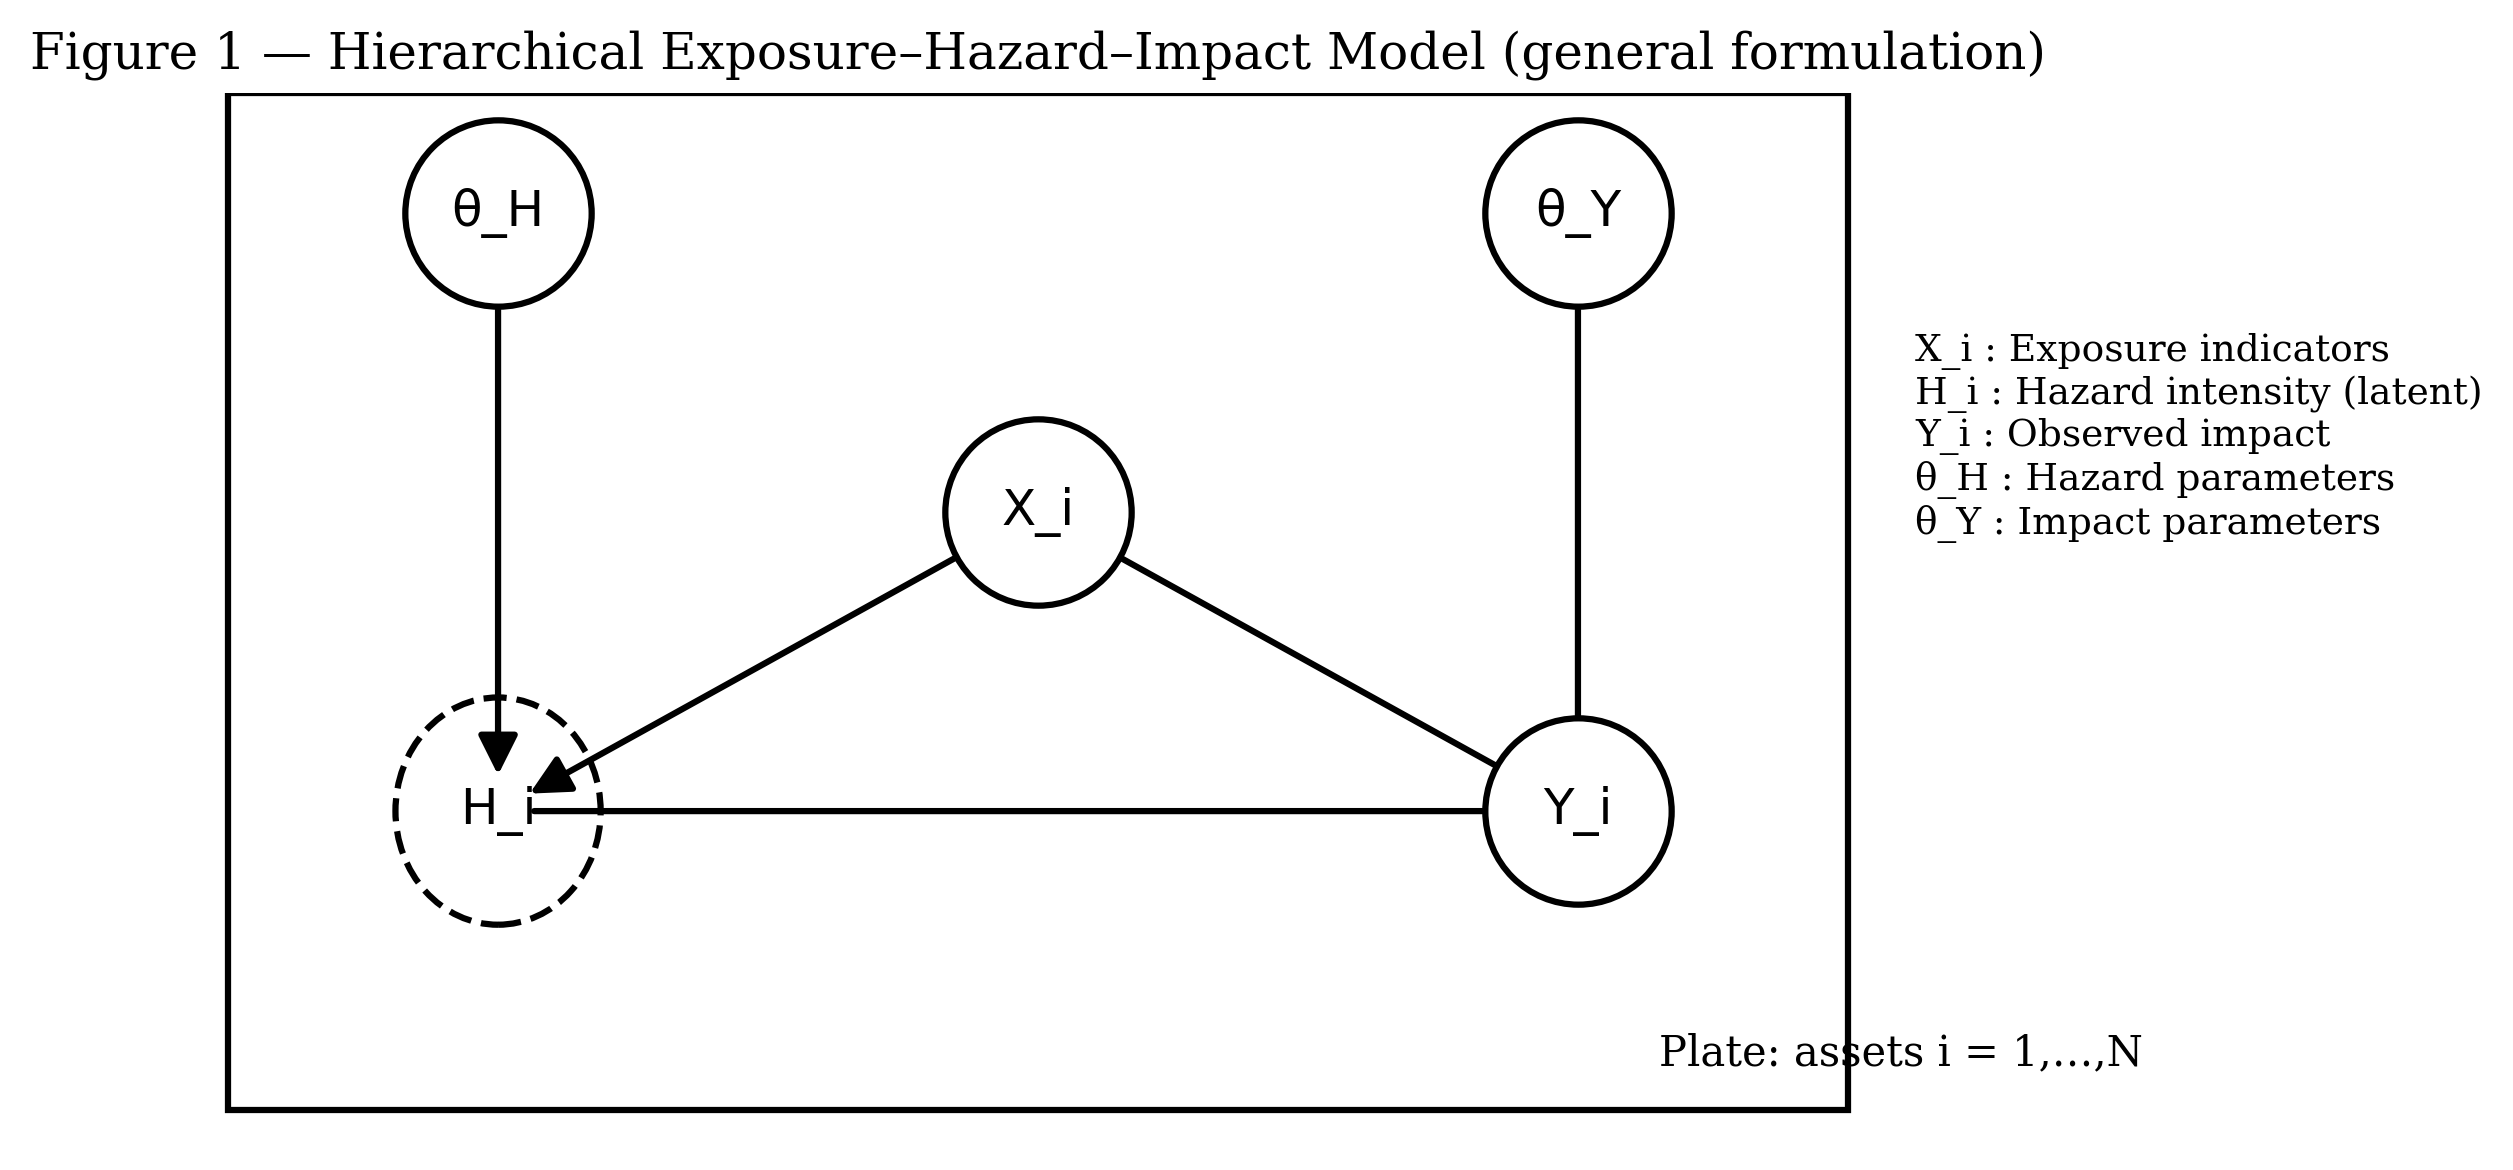
\includegraphics[keepaspectratio,alt={Hierarchical exposure--hazard--impact model}]{figures/fig01_graphical_model.png}}
\caption{Hierarchical exposure--hazard--impact model}
\end{figure}

Figure 1 illustrates the hierarchical exposure--hazard--impact structure
underlying the model.

\subsection{Decision stability
concept}\label{decision-stability-concept}

\begin{figure}
\centering
\pandocbounded{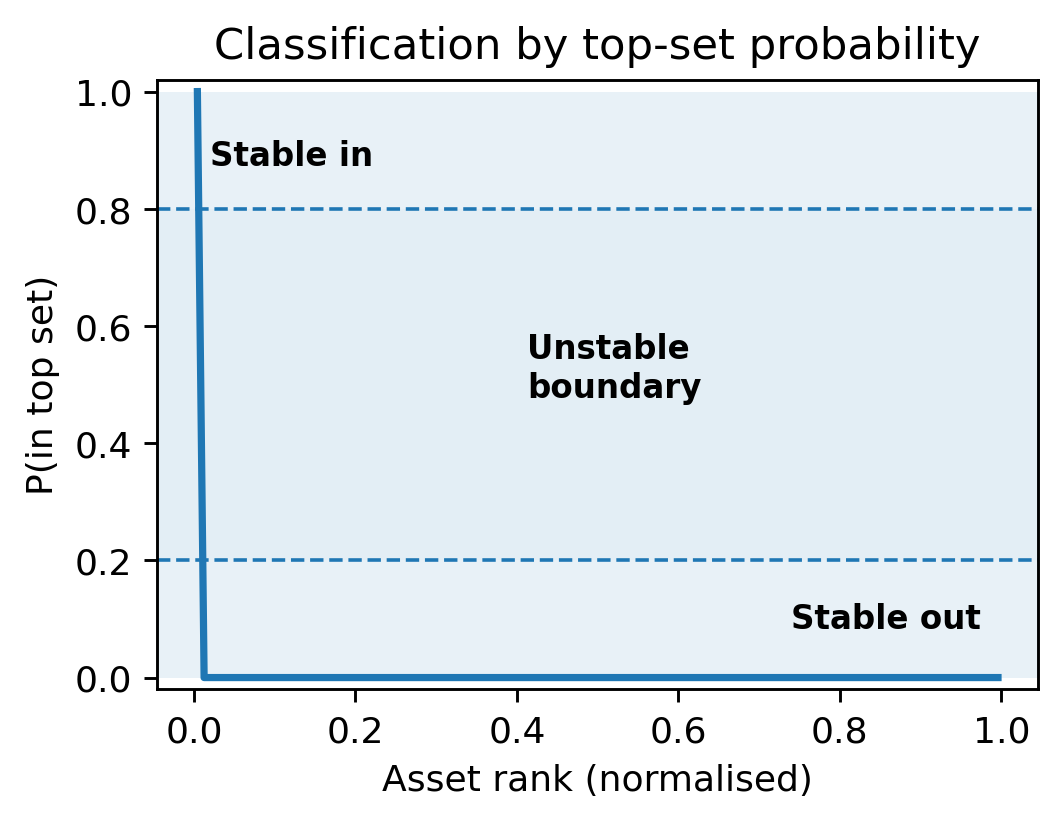
\includegraphics[keepaspectratio,alt={Classification of stable and unstable prioritisation regions}]{figures/RTM_03_stability_classification.png}}
\caption{Classification of stable and unstable prioritisation regions}
\end{figure}

Figure 2 illustrates the central decision structure explored in the
paper. Most assets exhibit stable prioritisation behaviour with
posterior top-k membership probabilities close to either 0 or 1. Only a
narrow intermediate boundary region exhibits unstable prioritisation
behaviour under posterior uncertainty.

\subsection{Cross-city transfer
concept}\label{cross-city-transfer-concept}

\begin{figure}
\centering
\pandocbounded{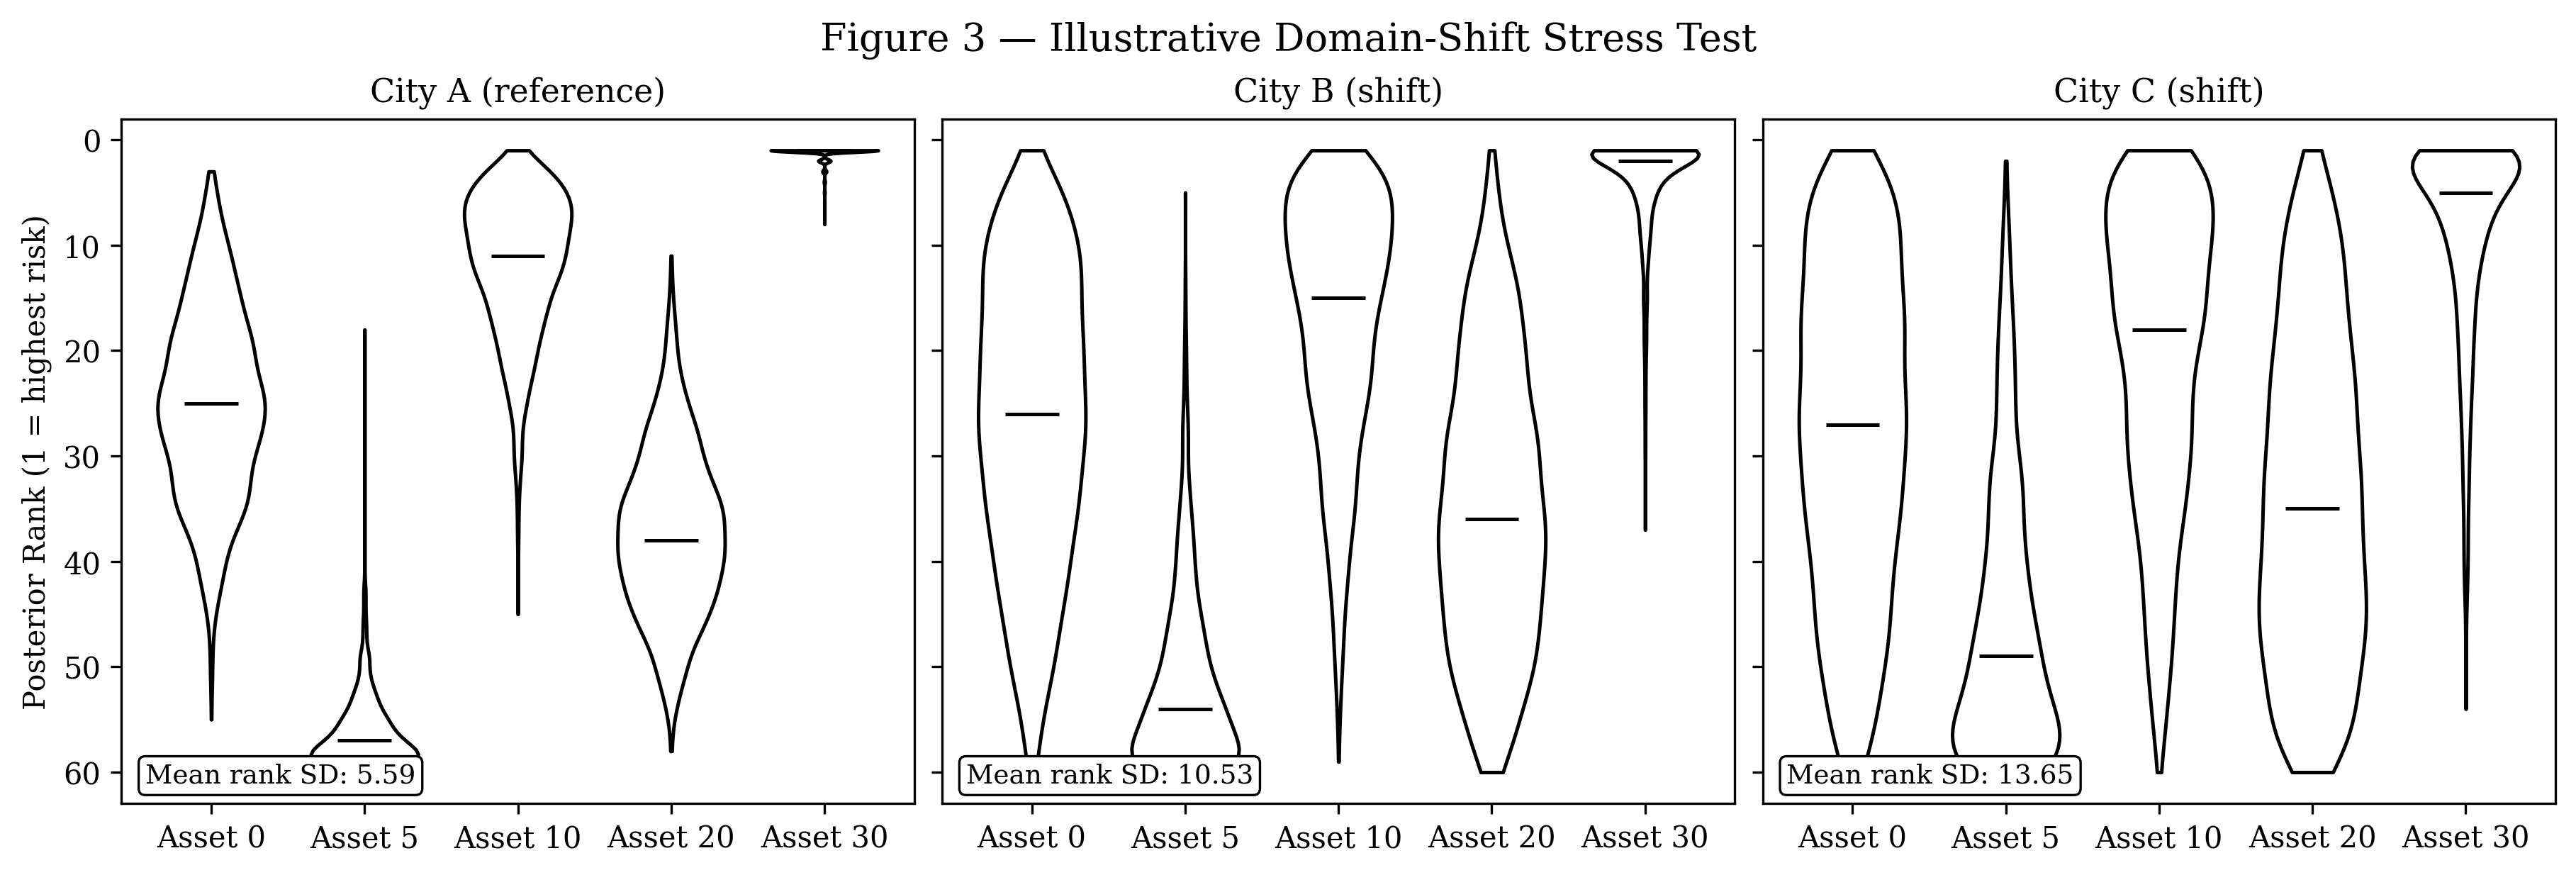
\includegraphics[keepaspectratio,alt={Cross-city transfer concept}]{figures/fig03_domain_shift_illustrative.png}}
\caption{Cross-city transfer concept}
\end{figure}

Figure 3 illustrates the fixed-specification transfer experiment. The
model specification, priors, feature definitions, and scaling remain
fixed while the framework is applied across different cities. Under
distributional shift, ranking variability may increase locally near the
prioritisation boundary.

\begin{center}\rule{0.5\linewidth}{0.5pt}\end{center}

\section{3. Experimental Design}\label{experimental-design}

\subsection{3.1 Phase 1 --- Rotterdam
baseline}\label{phase-1-rotterdam-baseline}

The baseline implementation is performed using Rotterdam as the
reference study area (\textasciitilde221,324 buildings).

Exposure is represented using hydrographic proximity indicators
including distance to water and local water density aggregation. Hazard
is represented using an ERA5-derived pluvial precipitation proxy.

A synthetic Bernoulli outcome variable is used in order to isolate the
behaviour of the probabilistic inference-to-decision pipeline from
empirical calibration challenges.

Posterior-derived decision metrics are computed from posterior draws
rather than deterministic risk scores.

\subsection{3.2 Phase 2 --- Hazard
perturbation}\label{phase-2-hazard-perturbation}

Robustness is evaluated through controlled perturbation of the hazard
proxy.

The standardised hazard representation is perturbed with additive
Gaussian noise while maintaining the same model structure and inference
procedure.

The objective is not to simulate physically realistic perturbations, but
to evaluate whether instability diffuses across the prioritisation
system under degraded hazard representation.

\subsection{3.3 Phase 3 --- Cross-city
transfer}\label{phase-3-cross-city-transfer}

The framework is transferred from Rotterdam to Hamburg and Donostia--San
Sebastián under fixed specification:

\begin{itemize}
\tightlist
\item
  same priors
\item
  same model structure
\item
  same feature definitions
\item
  same scaling reference
\item
  same decision metrics
\end{itemize}

Rotterdam statistics are retained as the scaling reference for
transferred cities.

The objective is not predictive optimisation for each city individually,
but evaluation of whether the decision-stability structure persists
under fixed specification and distributional shift.

\begin{center}\rule{0.5\linewidth}{0.5pt}\end{center}

\section{4. Bayesian Model}\label{bayesian-model}

The model defines a simple generative structure linking exposure, hazard
proxy, and binary impact outcome.

Asset-level impact probability is modelled using a logistic regression
structure:

\[
p_i =
\operatorname{logit}^{-1}
\left(
\alpha + \beta_E E_i + \beta_H H_i
\right)
\]

\[
Y_i \sim \operatorname{Bernoulli}(p_i)
\]

where:

\begin{itemize}
\tightlist
\item
  \(E_i\) denotes the exposure proxy
\item
  \(H_i\) denotes the hazard proxy
\item
  \(Y_i \in \{0,1\}\) denotes the impact indicator
\end{itemize}

\subsection{Priors}\label{priors}

Weakly informative priors are assigned to model parameters:

\[
\alpha, \beta_E, \beta_H \sim \mathcal{N}(0, 2.5)
\]

\subsection{Inference}\label{inference}

Posterior inference is performed using PyMC with Hamiltonian Monte Carlo
sampling through the NUTS sampler.

Inference is performed using:

\begin{itemize}
\tightlist
\item
  4 chains
\item
  1000 tuning iterations
\item
  1000 posterior draws per chain
\item
  \texttt{target\_accept\ =\ 0.9}
\end{itemize}

Diagnostics include:

\begin{itemize}
\tightlist
\item
  \(\hat{R}\) convergence diagnostics
\item
  effective sample size (ESS)
\item
  prior predictive checks
\item
  posterior predictive checks
\end{itemize}

\subsection{Prior predictive
validation}\label{prior-predictive-validation}

Prior predictive checks were used to verify that the prior specification
does not imply implausibly high citywide event rates before observing
the synthetic outcome data.

\begin{figure}
\centering
\pandocbounded{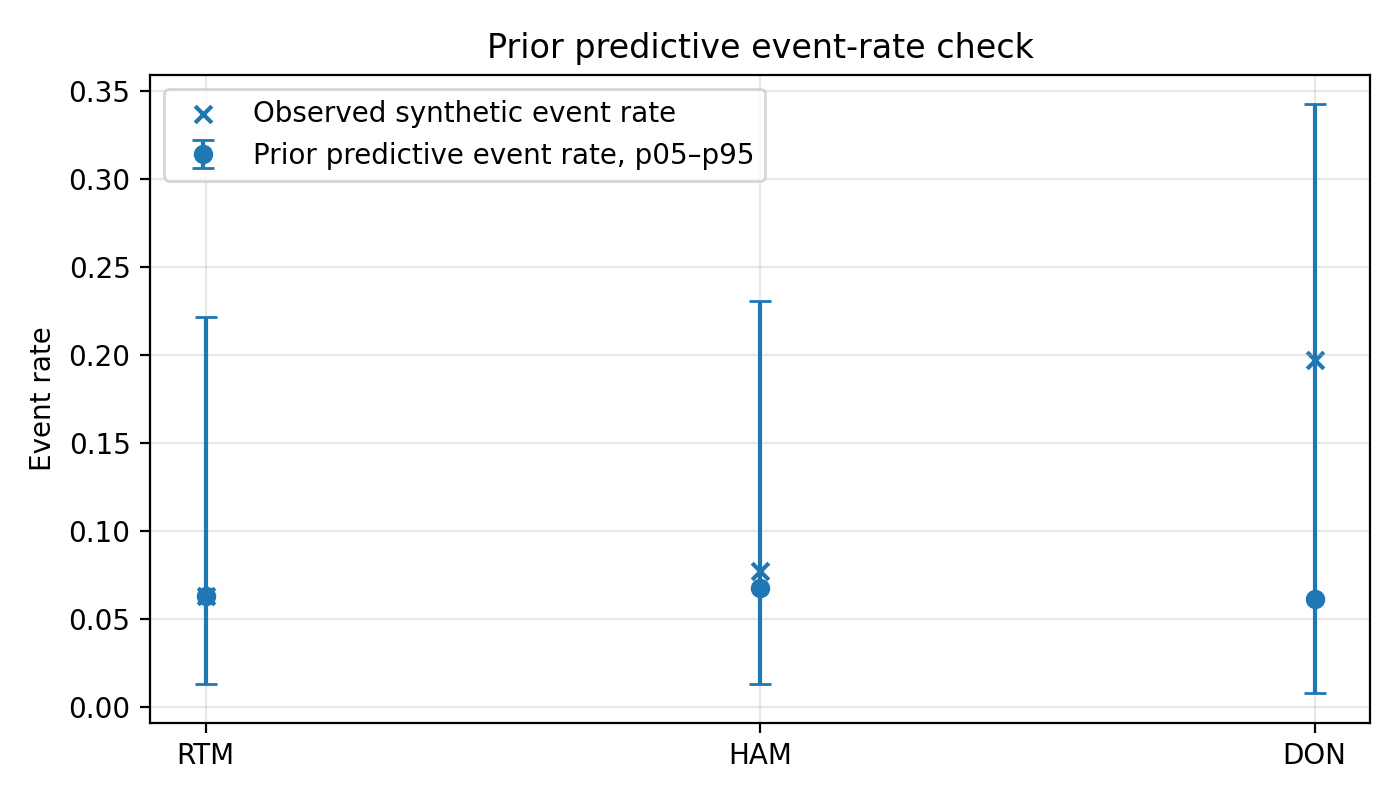
\includegraphics[keepaspectratio,alt={Prior predictive event-rate check}]{figures/fig_prior_predictive_event_rate.png}}
\caption{Prior predictive event-rate check}
\end{figure}

The prior predictive distribution remains compatible with low baseline
event rates while still allowing uncertainty across cities. This
supports the use of the prior specification as a weakly informative
baseline rather than an implicit high-risk assumption.

All reported models achieved stable convergence behaviour under the
current specification.

\subsection{Model scope}\label{model-scope}

The logistic specification is intentionally minimal, serving as a
baseline to isolate the behaviour of posterior-derived decision metrics
rather than to optimise predictive performance.

The present results should therefore not be interpreted as hydraulic
validation or operational flood prediction.

\begin{center}\rule{0.5\linewidth}{0.5pt}\end{center}

\section{5. Posterior-Derived Decision
Metrics}\label{posterior-derived-decision-metrics}

Rather than relying on point estimates, prioritisation decisions are
derived directly from posterior draws.

For each posterior draw:

\begin{enumerate}
\def\labelenumi{\arabic{enumi}.}
\tightlist
\item
  asset-level impact probabilities are computed
\item
  assets are ranked
\item
  the top-k subset is extracted
\end{enumerate}

This produces a posterior distribution over prioritisation membership
rather than a single deterministic ranking.

\subsection{Posterior mean risk}\label{posterior-mean-risk}

\[
p_{\text{mean}, i}
=
\mathbb{E}_{p(\theta \mid \text{data})}
\left[
P(Y_i = 1 \mid \theta)
\right]
\]

\subsection{Top-k membership
probability}\label{top-k-membership-probability}

For a prioritisation threshold \(k\), the probability that asset \(i\)
belongs to the top-k highest risk assets is:

\[
P(i \in \text{Top}_k \mid \text{posterior})
\]

This quantity forms the primary inferential object of the analysis.

\subsection{Borderline share}\label{borderline-share}

Borderline share is defined as:

\[
0.2 < P(i \in \text{Top}_k) < 0.8
\]

These assets form the prioritisation boundary where decision outcomes
remain unstable under posterior uncertainty.

\begin{center}\rule{0.5\linewidth}{0.5pt}\end{center}

\section{6. Results}\label{results}

\subsection{6.1 Rotterdam baseline}\label{rotterdam-baseline}

Figure 4 shows the empirical cumulative distribution of posterior mean
impact probabilities across Rotterdam.

\begin{figure}
\centering
\pandocbounded{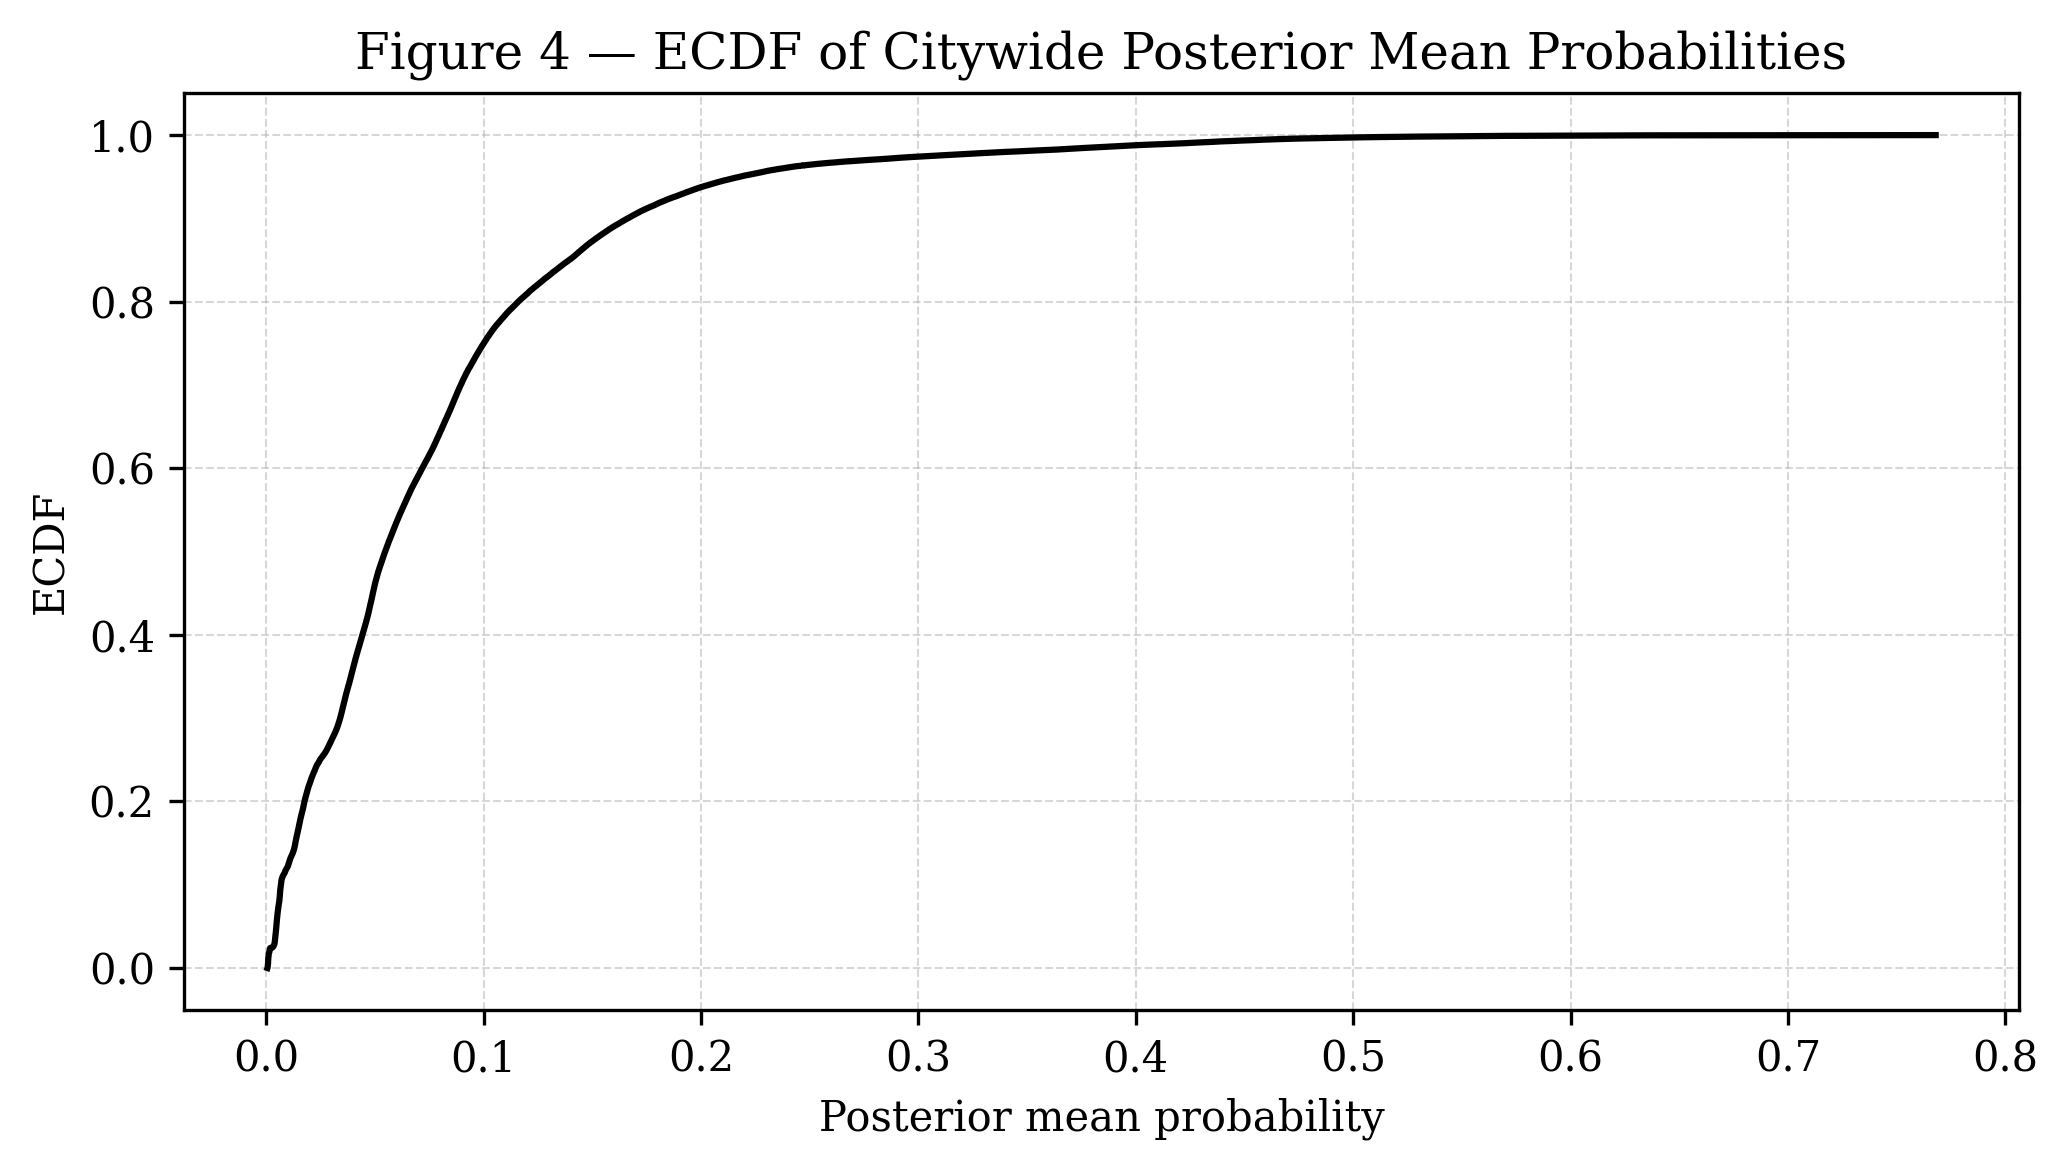
\includegraphics[keepaspectratio,alt={Empirical cumulative distribution of posterior mean probabilities}]{figures/fig04_pmean_city_ecdf.png}}
\caption{Empirical cumulative distribution of posterior mean
probabilities}
\end{figure}

Posterior mean probabilities are strongly concentrated near low values,
while only a small subset of assets occupy the upper tail of the
distribution.

Decision stability is evaluated through posterior-derived top-k
membership probabilities. Figure 5 shows that, across prioritisation
thresholds, borderline share remains extremely small relative to the
total asset population.

\begin{figure}
\centering
\pandocbounded{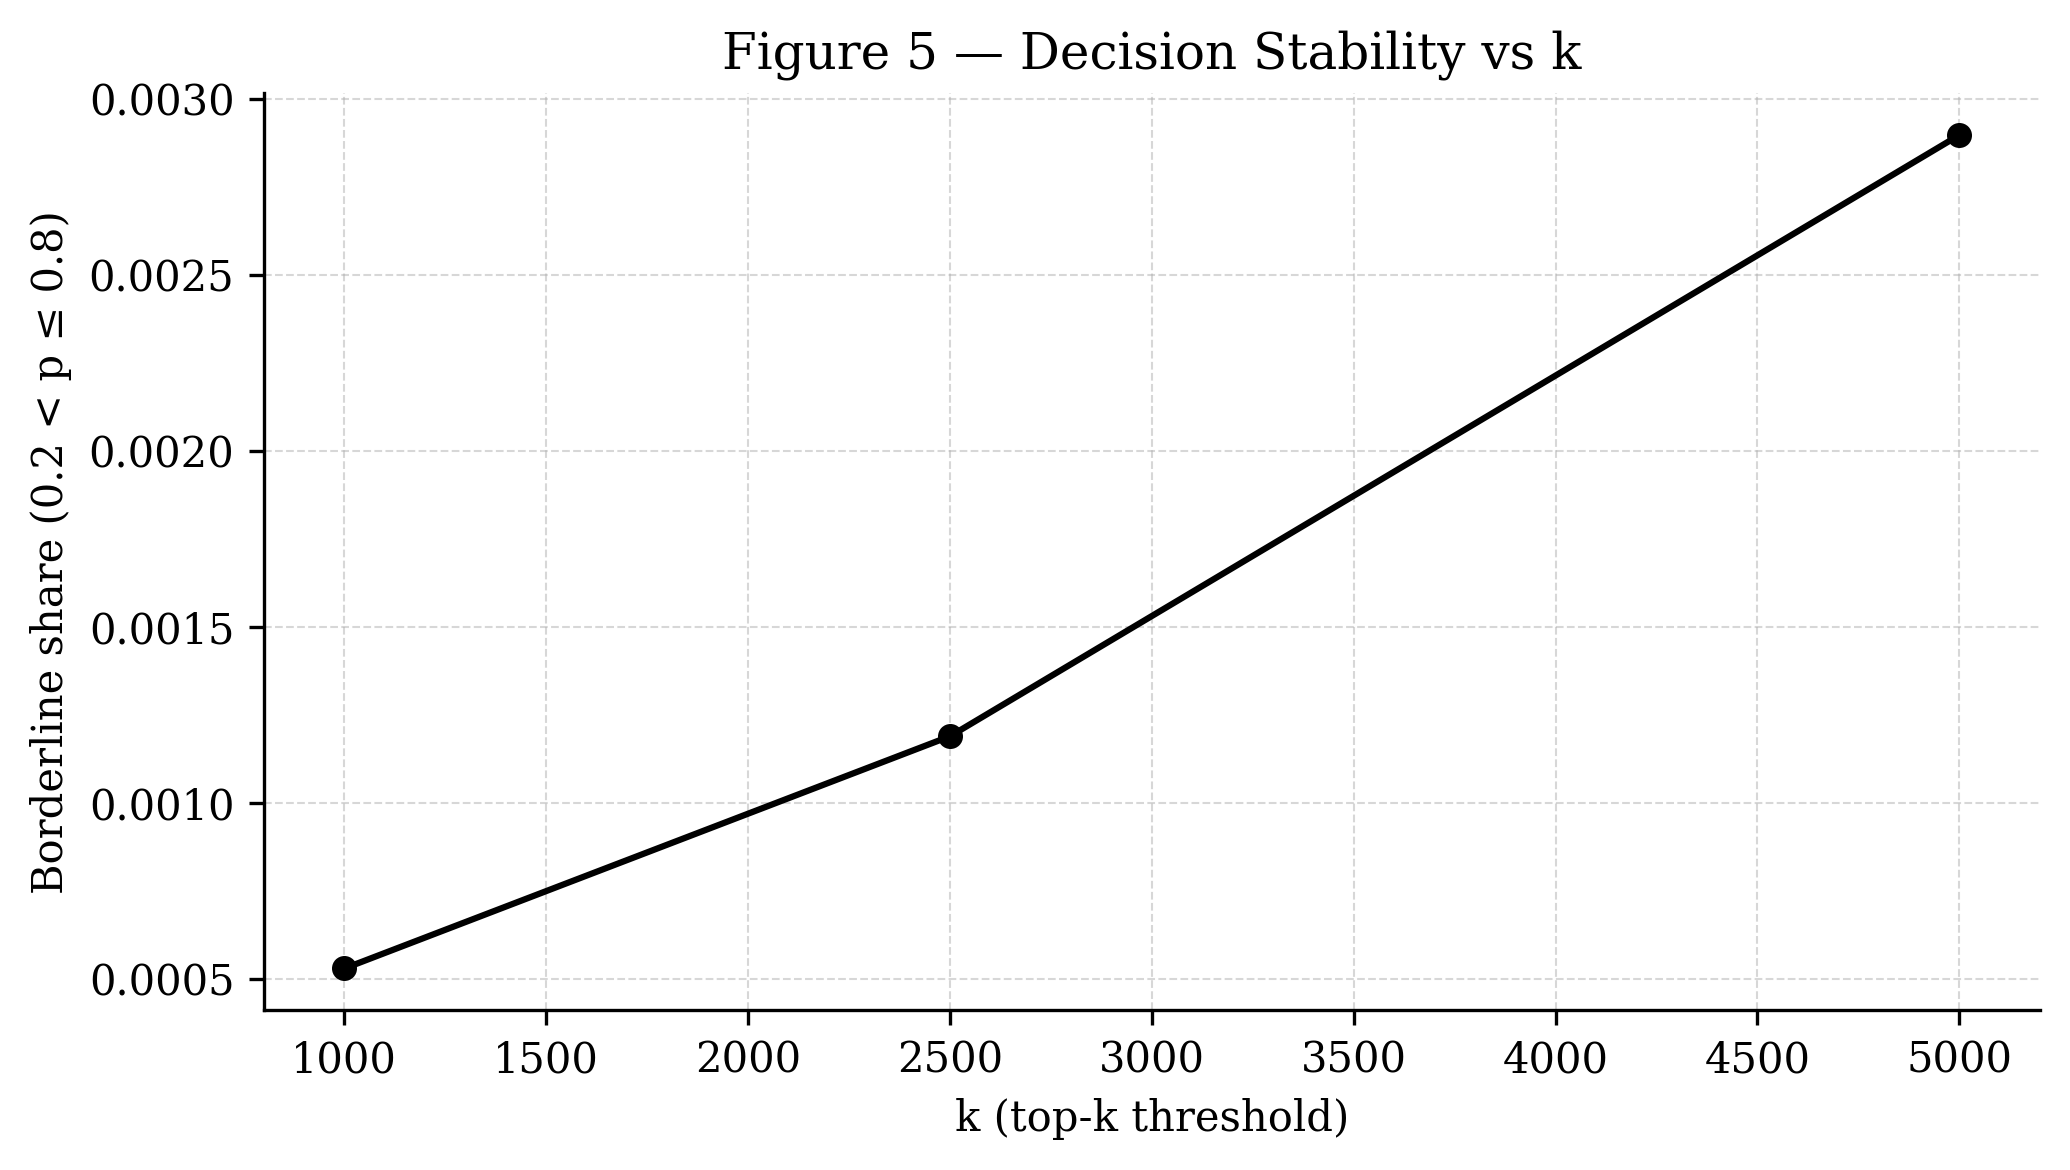
\includegraphics[keepaspectratio,alt={Borderline share across prioritisation thresholds}]{figures/fig05_borderline_vs_k.png}}
\caption{Borderline share across prioritisation thresholds}
\end{figure}

For the Top-1000 prioritisation threshold, most assets exhibit highly
polarised membership probabilities close to either 0 or 1.

Figure 6 illustrates the deterministic ranking structure induced by
posterior mean risk estimates.

\begin{figure}
\centering
\pandocbounded{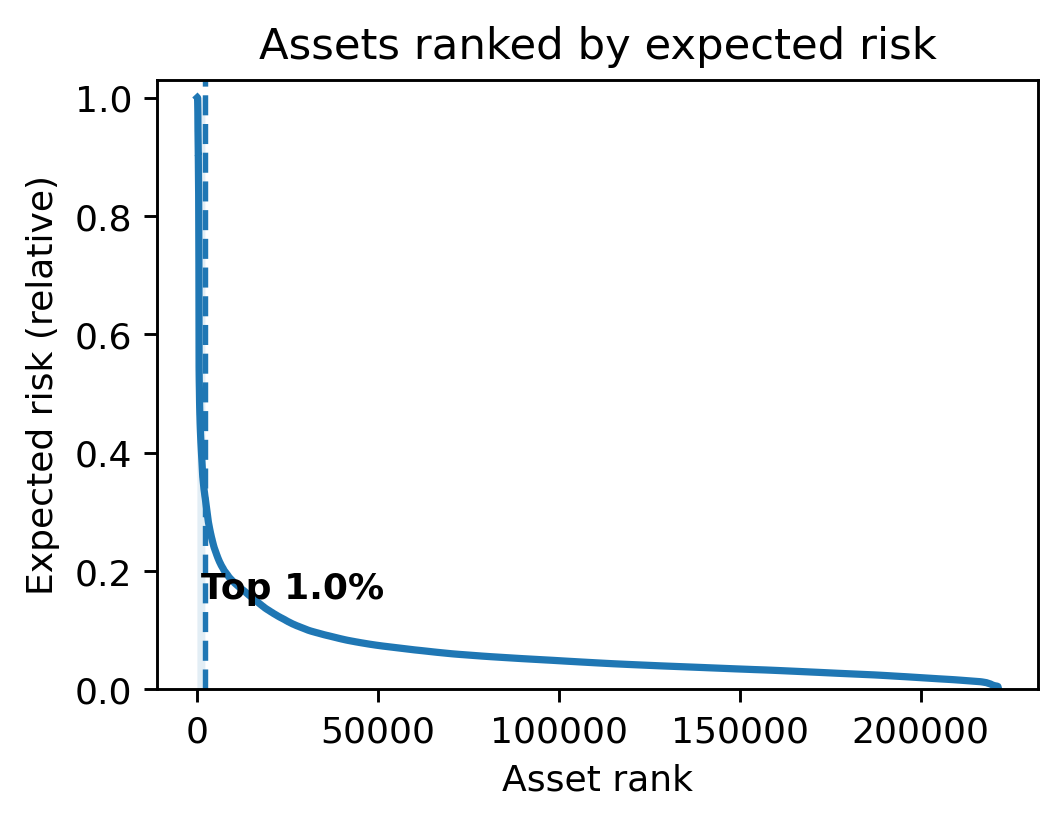
\includegraphics[keepaspectratio,alt={Deterministic ranking structure}]{figures/RTM_01_deterministic_ranking.png}}
\caption{Deterministic ranking structure}
\end{figure}

A small subset of assets occupies the upper tail of the prioritisation
distribution, while the majority of assets exhibit substantially lower
expected risk values. This concentration motivates the use of top-k
prioritisation analysis under posterior uncertainty.

Figure 7 shows posterior top-k membership probability as a function of
asset rank.

\begin{figure}
\centering
\pandocbounded{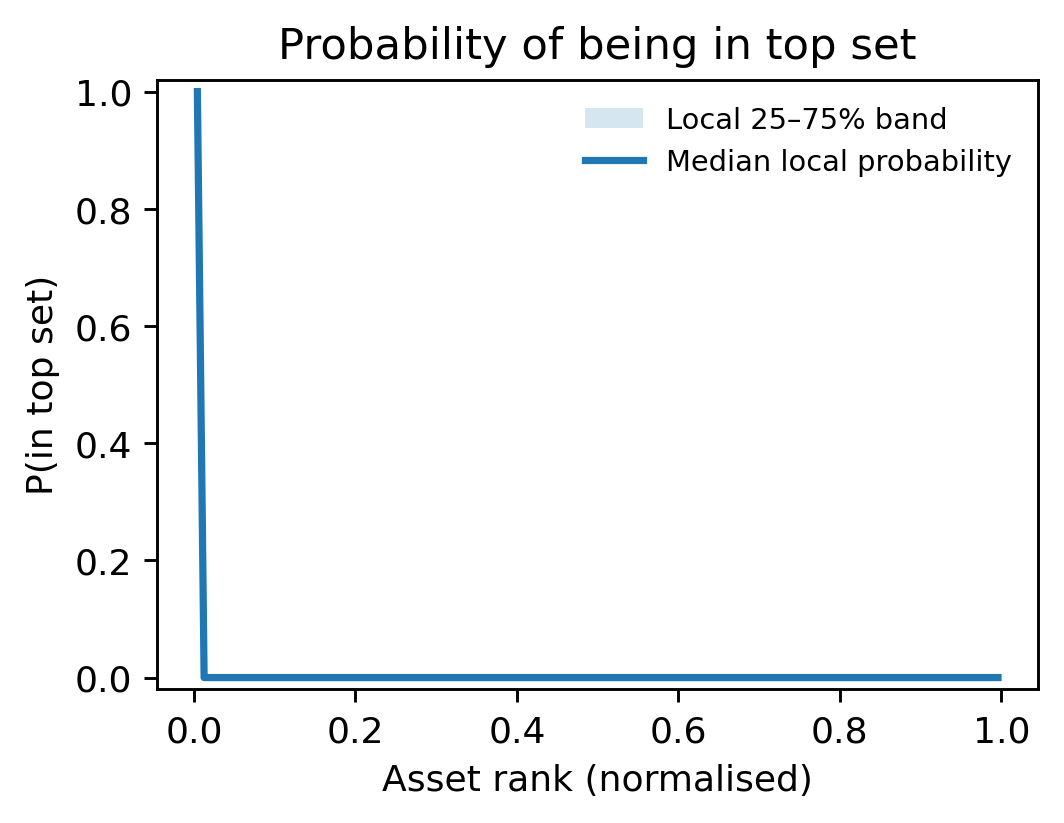
\includegraphics[keepaspectratio,alt={Posterior top-k membership probability structure}]{figures/RTM_02_probability_ranking.png}}
\caption{Posterior top-k membership probability structure}
\end{figure}

Most assets exhibit highly stable prioritisation behaviour with
probabilities close to either 0 or 1. Only a very narrow boundary region
exhibits intermediate membership probabilities, indicating localised
instability rather than diffuse uncertainty across the prioritisation
system.

\subsection{Posterior predictive
checks}\label{posterior-predictive-checks}

Figure 8 shows the posterior predictive check for the Rotterdam baseline
model.

\begin{figure}
\centering
\pandocbounded{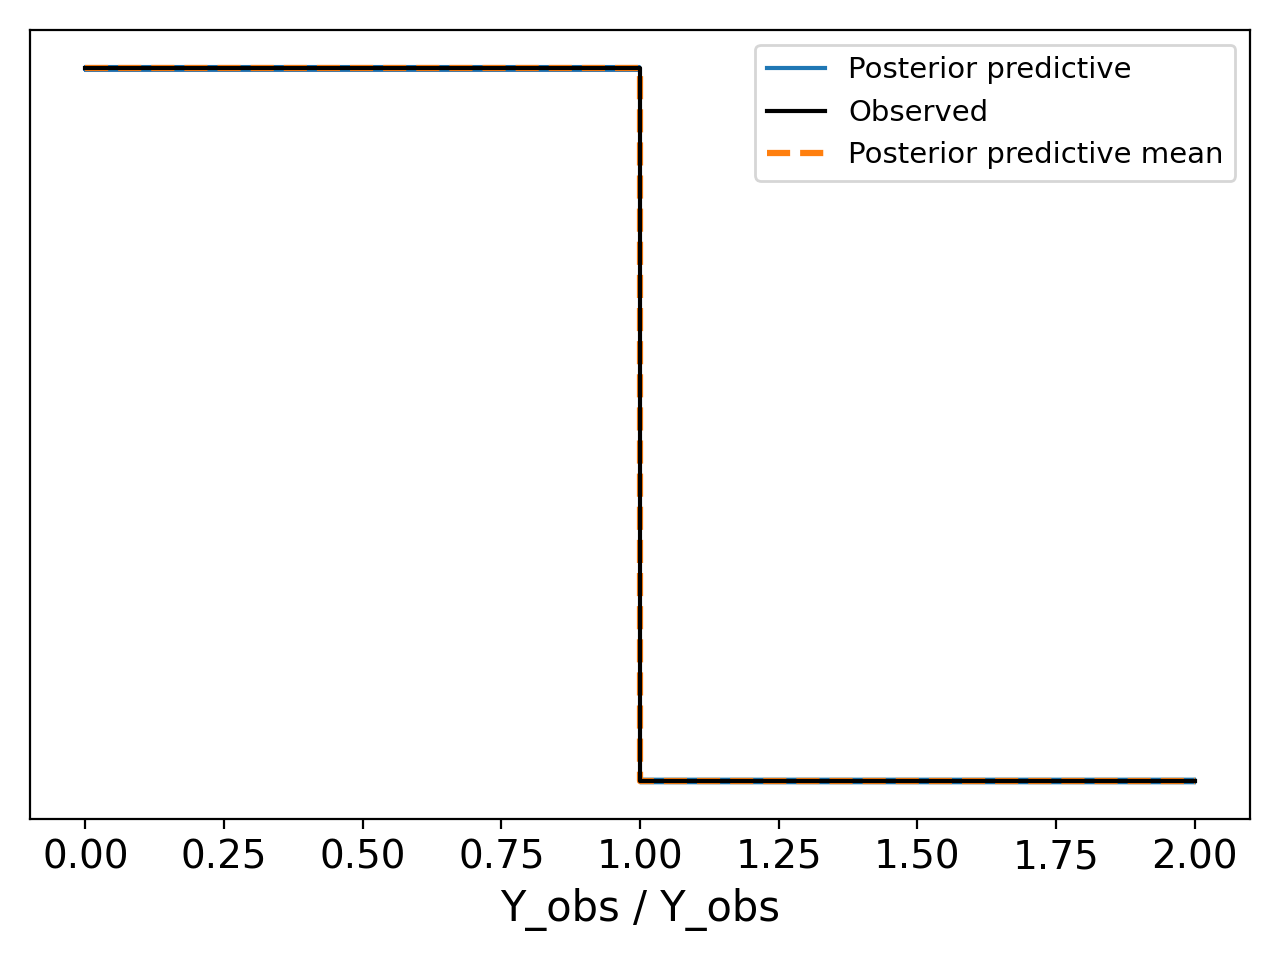
\includegraphics[keepaspectratio,alt={Posterior predictive check for Rotterdam}]{figures/ppc_RTM.png}}
\caption{Posterior predictive check for Rotterdam}
\end{figure}

The posterior predictive distribution remains closely aligned with the
observed synthetic outcome distribution, suggesting stable inference
behaviour under the current baseline formulation.

\begin{center}\rule{0.5\linewidth}{0.5pt}\end{center}

\subsection{6.2 Robustness to hazard
perturbation}\label{robustness-to-hazard-perturbation}

To evaluate whether the observed concentration of instability depends on
deterministic hazard specification, controlled perturbations are
introduced into the standardised hazard representation:

\[
H_i^{\text{perturbed}} = H_i + \epsilon_i,
\quad
\epsilon_i \sim \mathcal{N}(0, \sigma)
\]

The following perturbation levels are evaluated:

\begin{itemize}
\tightlist
\item
  \(\sigma = 0.00\)
\item
  \(\sigma = 0.05\)
\item
  \(\sigma = 0.10\)
\item
  \(\sigma = 0.20\)
\item
  \(\sigma = 0.30\)
\end{itemize}

{\def\LTcaptype{none} % do not increment counter
\begin{longtable}[]{@{}lr@{}}
\toprule\noalign{}
\(\sigma\) & Borderline Share \\
\midrule\noalign{}
\endhead
\bottomrule\noalign{}
\endlastfoot
0.00 & 0.0158 \\
0.05 & 0.0130 \\
0.10 & 0.0148 \\
0.20 & 0.0172 \\
0.30 & 0.0174 \\
\end{longtable}
}

Figure 9 shows that increasing hazard perturbation does not produce
diffuse instability across the system. Instead, instability remains
concentrated near the prioritisation boundary across all tested
perturbation levels.

\begin{figure}
\centering
\pandocbounded{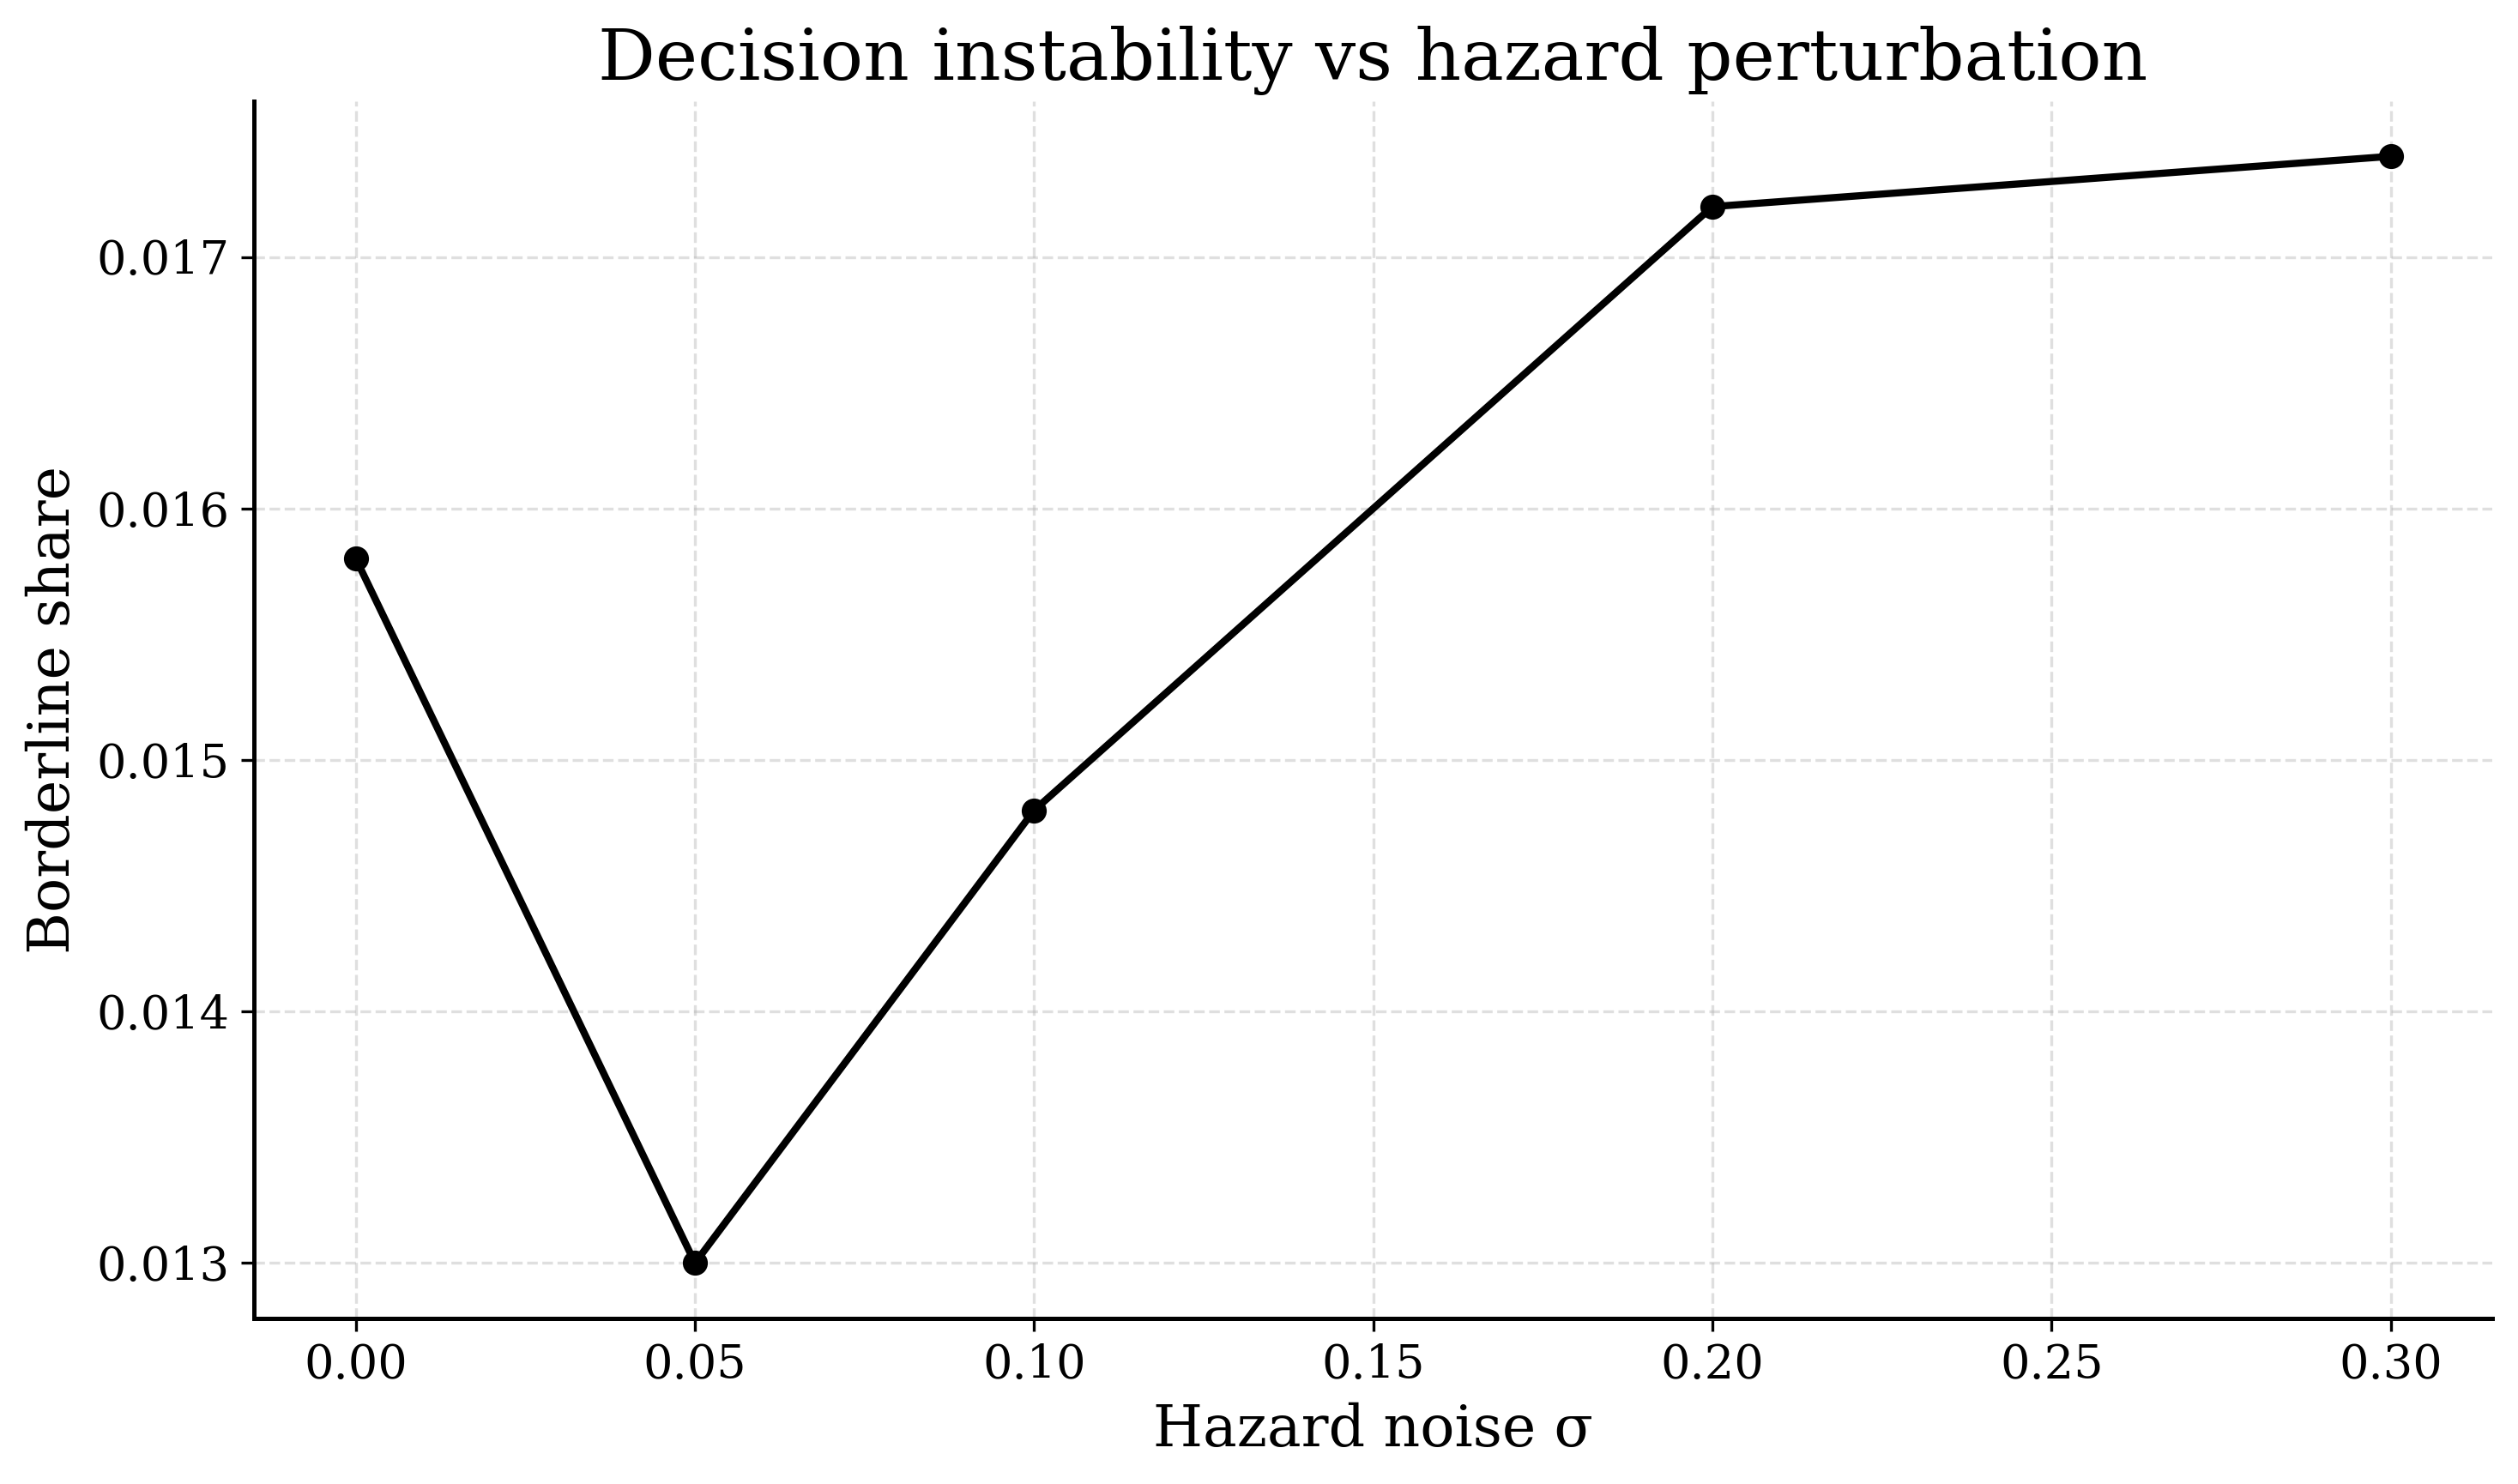
\includegraphics[keepaspectratio,alt={Decision instability under hazard perturbation}]{figures/fig07_borderline_vs_sigma.png}}
\caption{Decision instability under hazard perturbation}
\end{figure}

\begin{center}\rule{0.5\linewidth}{0.5pt}\end{center}

\subsection{6.3 Cross-city transfer}\label{cross-city-transfer}

The same framework is applied to Hamburg and Donostia--San Sebastián
under fixed specification.

\subsubsection{Rotterdam → Hamburg}\label{rotterdam-hamburg}

The Hamburg transfer exhibits decision behaviour similar to the
Rotterdam baseline. Top-k membership probabilities remain strongly
polarised and borderline share remains negligible across evaluated
prioritisation thresholds.

The concentration of instability near the prioritisation boundary
therefore remains structurally preserved under transfer.

\subsubsection{Rotterdam → Donostia--San
Sebastián}\label{rotterdam-donostiasan-sebastiuxe1n}

Donostia--San Sebastián exhibits moderate broadening of the unstable
prioritisation boundary consistent with distributional shift, while
overall instability remains spatially concentrated.

Figure 10 compares borderline share across cities and top-k thresholds
under fixed-specification transfer.

\begin{figure}
\centering
\pandocbounded{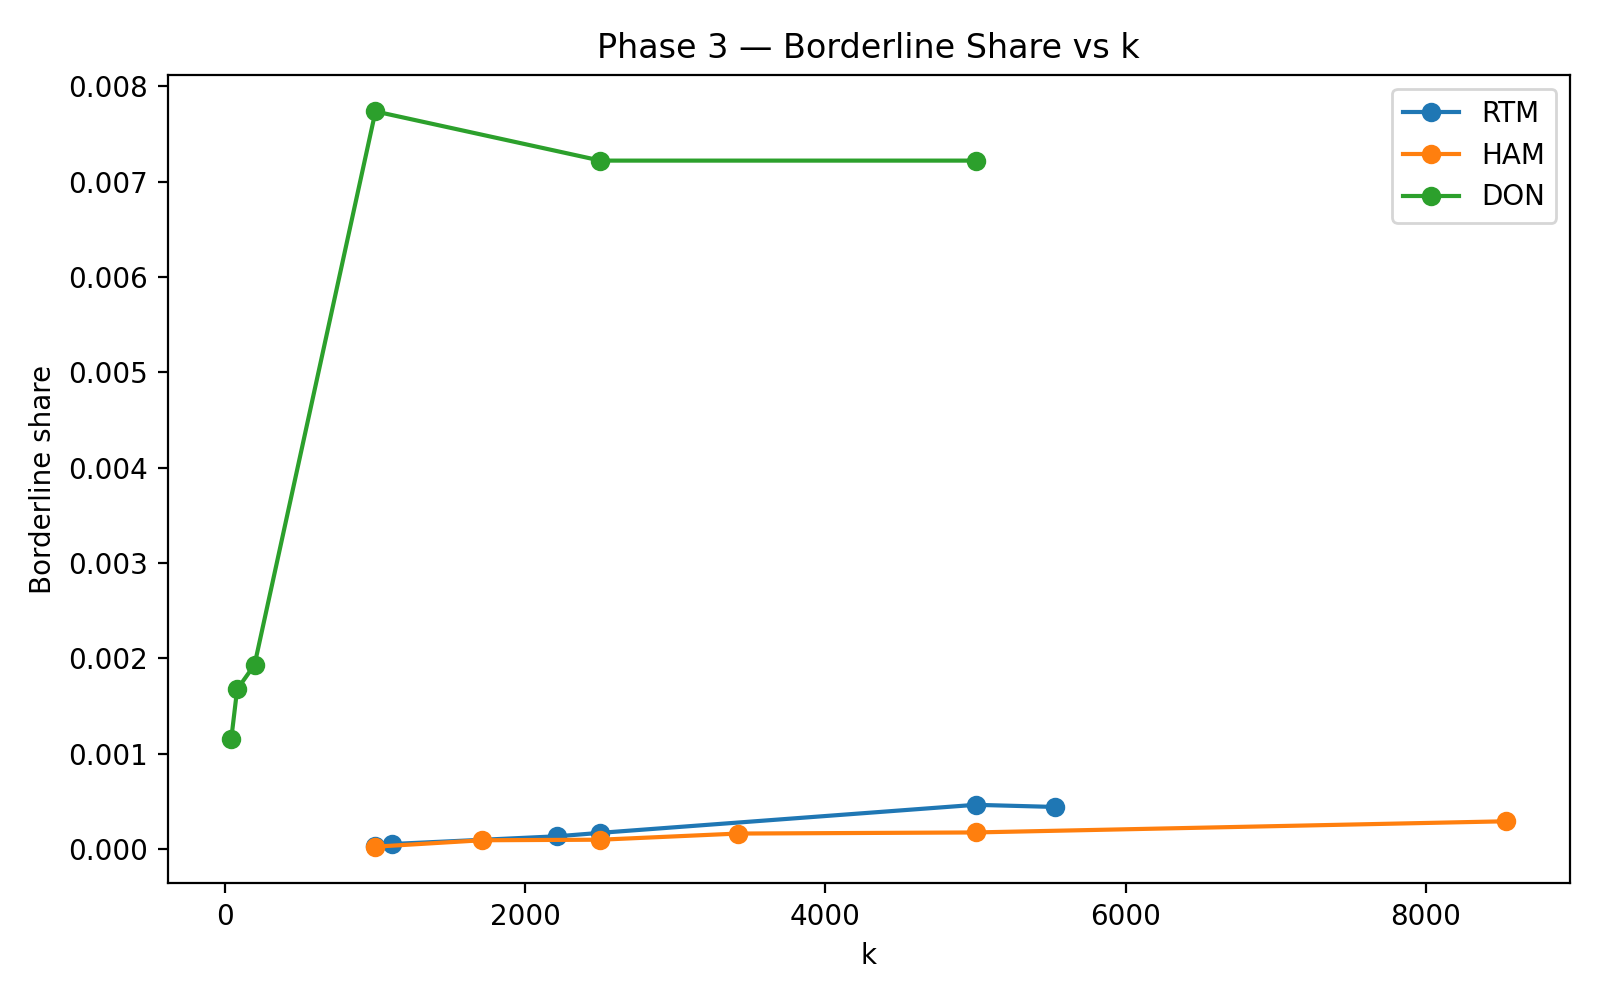
\includegraphics[keepaspectratio,alt={Borderline share under fixed-specification transfer}]{figures/phase3_borderline_share_vs_k.png}}
\caption{Borderline share under fixed-specification transfer}
\end{figure}

{\def\LTcaptype{none} % do not increment counter
\begin{longtable}[]{@{}lrrr@{}}
\toprule\noalign{}
City & Representative k & Assets & Borderline share \\
\midrule\noalign{}
\endhead
\bottomrule\noalign{}
\endlastfoot
RTM & 1000 & 221,324 & 0.0036\% \\
HAM & 1000 & 341,530 & 0.0026\% \\
DON & 1000 & 7,755 & 0.7737\% \\
DON & 5000 & 7,755 & 0.7221\% \\
\end{longtable}
}

Table 1 summarises representative borderline-share values for each city
under transfer.

The table shows the main transfer result directly. Rotterdam and Hamburg
exhibit almost negligible borderline share, while Donostia--San
Sebastián shows a wider unstable boundary. However, even under this
stronger transfer stress, the borderline set remains below 1\% of
assets.

Figure 11 compares posterior top-k membership probability structure
across Rotterdam, Hamburg, and Donostia--San Sebastián under
fixed-specification transfer.

\begin{figure}
\centering
\pandocbounded{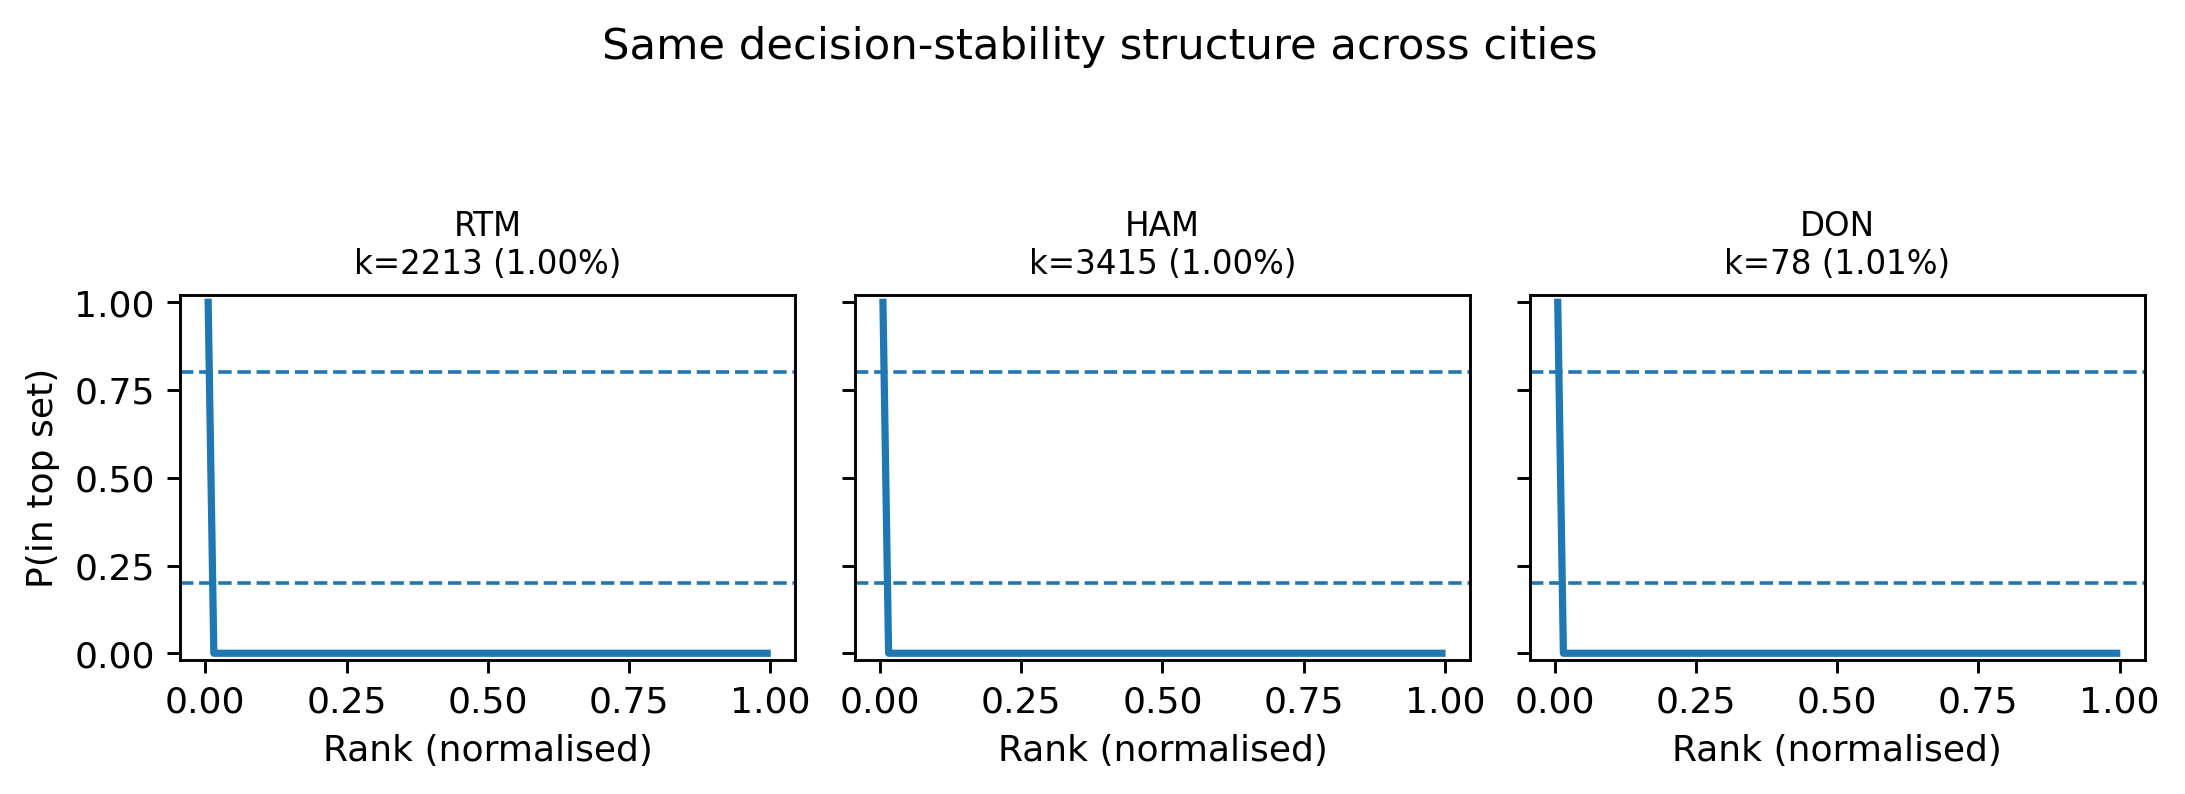
\includegraphics[keepaspectratio,alt={Cross-city posterior probability comparison}]{figures/04_cross_city_probability_structure.png}}
\caption{Cross-city posterior probability comparison}
\end{figure}

Across all three cities, posterior instability remains concentrated near
a narrow prioritisation boundary. Rotterdam and Hamburg exhibit highly
polarised membership structure, while Donostia--San Sebastián exhibits
moderate local broadening of the unstable boundary region consistent
with distributional shift.

Figures 12--14 show the spatial distribution of posterior top-k
membership probability for the Rotterdam reference case and the two
transferred cities.

\begin{figure}
\centering
\pandocbounded{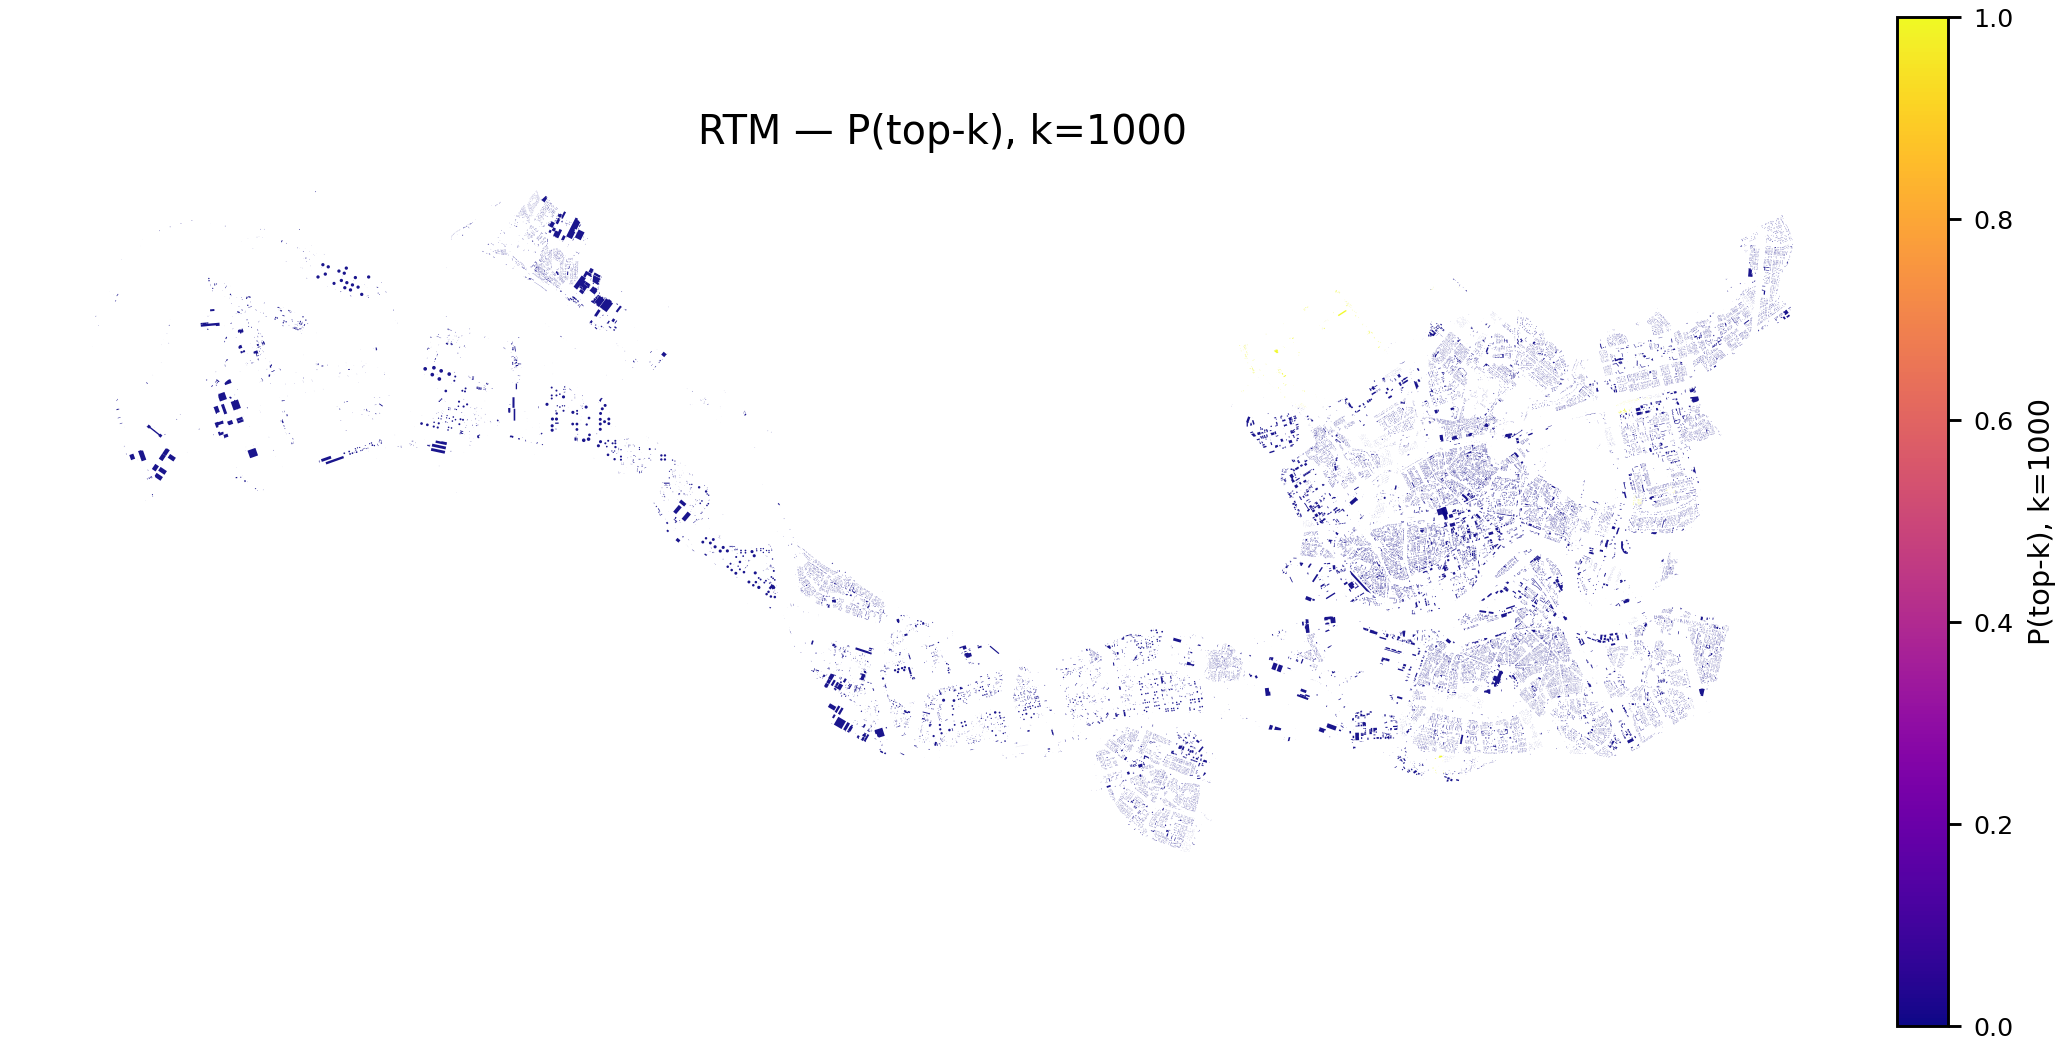
\includegraphics[keepaspectratio,alt={Rotterdam posterior top-k probability map, k = 1000}]{figures/RTM_topk_prob_k1000_map.png}}
\caption{Rotterdam posterior top-k probability map, k = 1000}
\end{figure}

\begin{figure}
\centering
\pandocbounded{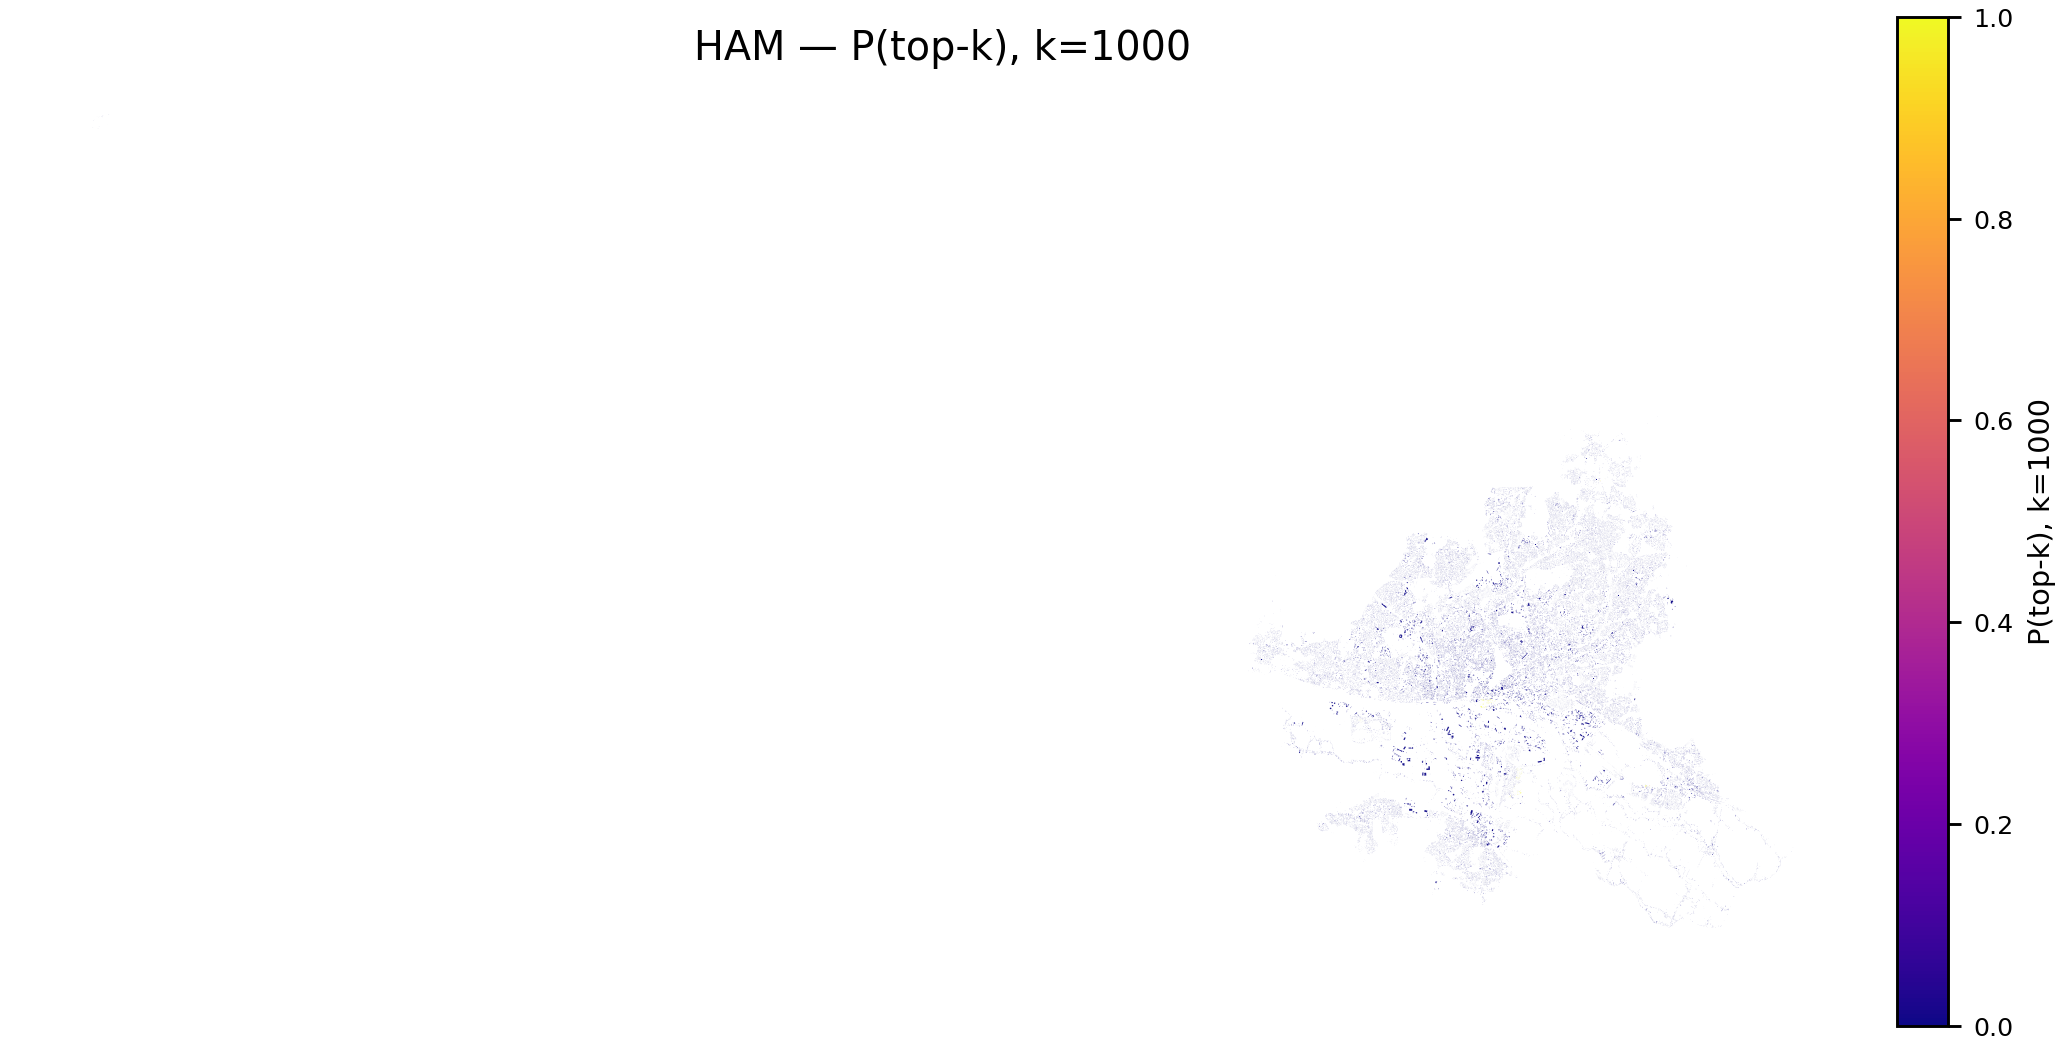
\includegraphics[keepaspectratio,alt={Hamburg posterior top-k probability map, k = 1000}]{figures/HAM_topk_prob_k1000_map.png}}
\caption{Hamburg posterior top-k probability map, k = 1000}
\end{figure}

\begin{figure}
\centering
\pandocbounded{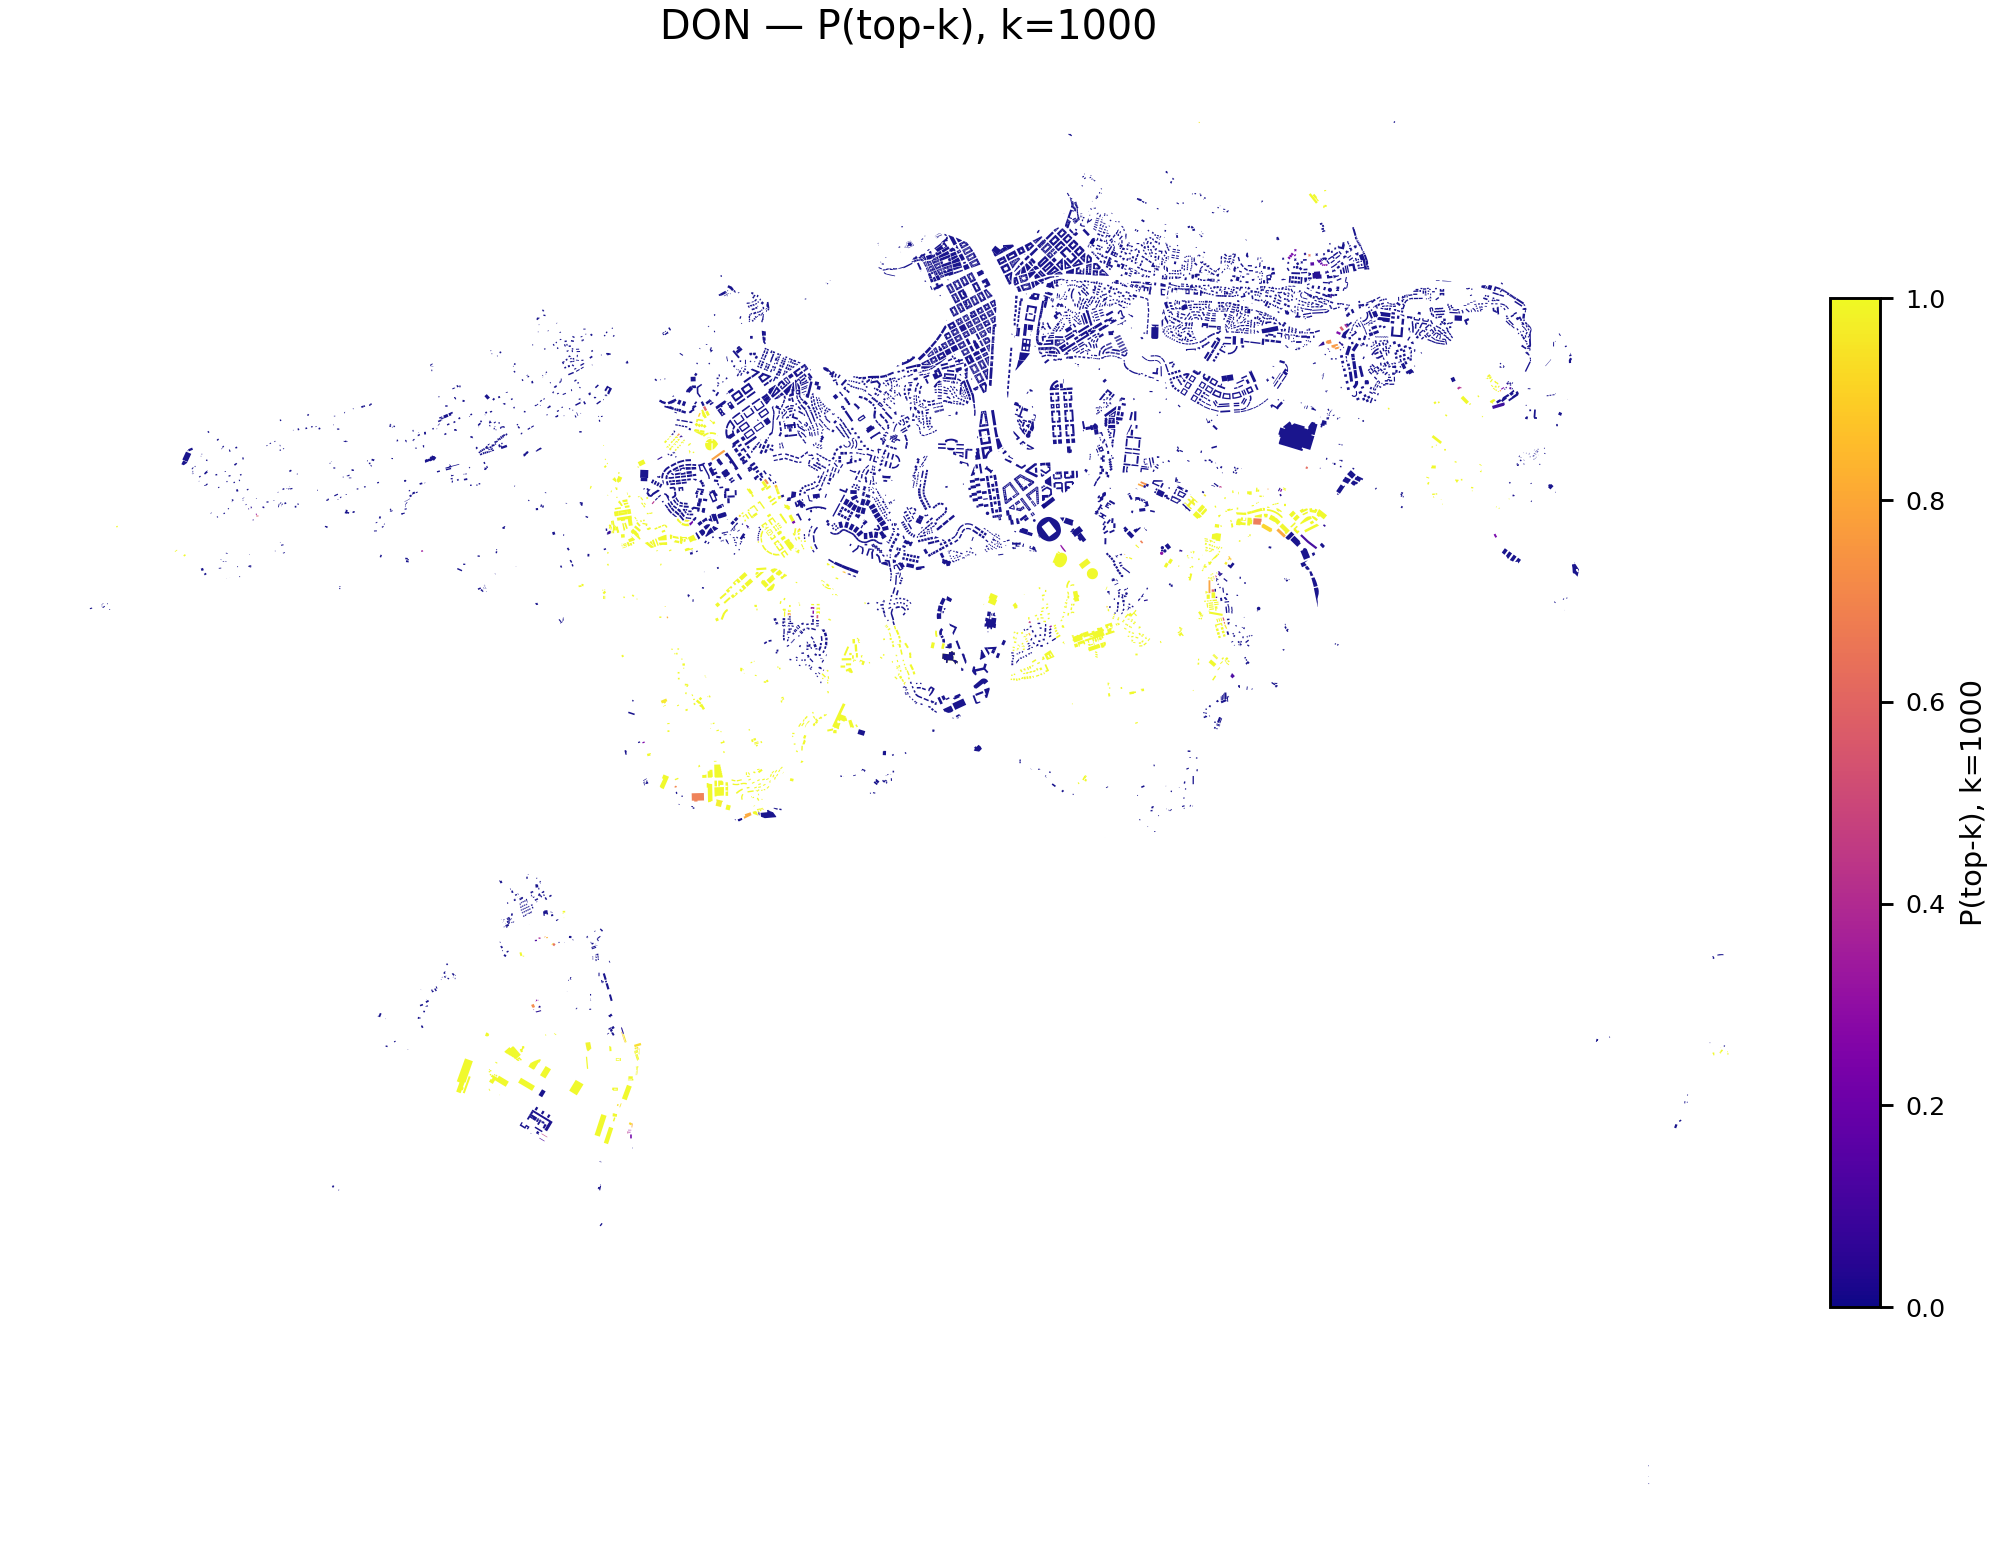
\includegraphics[keepaspectratio,alt={Donostia--San Sebastián posterior top-k probability map, k = 1000}]{figures/DON_topk_prob_k1000_map.png}}
\caption{Donostia--San Sebastián posterior top-k probability map, k =
1000}
\end{figure}

The Rotterdam and Hamburg maps show highly polarised posterior
membership structure, with most assets assigned probabilities close to
either 0 or 1. Donostia--San Sebastián exhibits increased local
fragmentation near the prioritisation boundary under fixed-specification
transfer. Despite this degradation, instability remains spatially
concentrated rather than diffuse across the system.

The transfer experiments suggest that the concentration of decision
instability near a narrow prioritisation boundary may represent a
structural property of the inference-to-decision pipeline rather than a
city-specific artefact.

\begin{center}\rule{0.5\linewidth}{0.5pt}\end{center}

\section{7. Discussion}\label{discussion}

This study demonstrates how prioritisation decisions can be analysed as
probabilistic objects rather than deterministic rankings.

By deriving decision metrics directly from posterior distributions, the
framework evaluates not only which assets appear most at risk, but also
how stable those prioritisation decisions remain under uncertainty
propagation.

Across baseline, perturbation, and transfer experiments, posterior
uncertainty remained concentrated near a relatively narrow
prioritisation boundary while the majority of assets exhibited stable
membership behaviour across posterior draws.

The perturbation experiments indicate that this structure is not highly
sensitive to moderate degradation in hazard representation. Similarly,
the transfer experiments suggest that the overall decision-stability
structure may persist under moderate distributional shift when the model
specification remains fixed.

The present results should not be interpreted as evidence of predictive
generalisation across cities. The experiments instead evaluate whether
posterior-derived decision behaviour remains structurally stable under
fixed-specification transfer.

Likewise, the framework evaluates stability of prioritisation under
uncertainty rather than correctness of prioritisation itself.

\begin{center}\rule{0.5\linewidth}{0.5pt}\end{center}

\section{8. Limitations}\label{limitations}

Several limitations should be noted.

\begin{itemize}
\tightlist
\item
  The hazard representation is proxy-based and does not model hydraulic
  flood dynamics.
\item
  The outcome variable is synthetic and not calibrated against observed
  damage data.
\item
  Exposure is represented using simplified hydrographic proximity
  indicators.
\item
  The current framework evaluates a single model family with limited
  prior sensitivity analysis.
\item
  The framework does not currently include latent hazard processes or
  utility-theoretic decision modelling.
\end{itemize}

These simplifications are intentional in the present baseline study in
order to isolate the statistical behaviour of posterior-derived
prioritisation metrics.

No claims of operational deployment or empirical flood prediction are
made.

\begin{center}\rule{0.5\linewidth}{0.5pt}\end{center}

\section{9. Conclusion}\label{conclusion}

This paper presented a Bayesian framework for analysing prioritisation
decision stability under uncertainty propagation.

Rather than treating rankings as deterministic outputs, the framework
derives posterior-based decision quantities that quantify uncertainty in
prioritisation membership itself.

Across baseline, perturbation, and transfer experiments, instability
remained concentrated near a narrow prioritisation boundary while most
assets exhibited stable prioritisation behaviour under posterior
uncertainty.

The contribution of the framework is methodological rather than
hydraulic.

The results demonstrate how posterior inference can be extended from
predictive estimation toward explicit analysis of prioritisation
stability under uncertainty.

\begin{center}\rule{0.5\linewidth}{0.5pt}\end{center}

\section{References}\label{references}

Hall, J. W., \& Harvey, H. (2009). Decision making under severe
uncertainties for flood risk management: A case study of Info-Gap
robustness analysis. \emph{Journal of Flood Risk Management}.

Lv, H., Wu, Z., Guan, X., \& Meng, Y. (2021). The construction of flood
loss ratio function in cities lacking loss data based on dynamic
proportional substitution and hierarchical Bayesian model. \emph{Journal
of Hydrology}.

McMillan, H., \& Brasington, J. (2008). End-to-end flood risk
assessment: A coupled model cascade with uncertainty estimation.
\emph{Water Resources Research}.

Mohor, G. S., et al.~(2021). Residential flood loss estimated from
Bayesian multilevel models. \emph{Natural Hazards and Earth System
Sciences}.

Sairam, N., Schröter, K., Rözer, V., Merz, B., \& Kreibich, H. (2019). A
Bayesian hierarchical model for flood damage estimation in data-scarce
regions. \emph{Water Resources Research}.

Wu, Y., et al.~(2019). Assessing urban flood disaster risk using
Bayesian network model and GIS applications. \emph{International Journal
of River Basin Management}.

Wu, Y., et al.~(2020). Urban flood disaster risk evaluation based on
ontology and Bayesian Network. \emph{Journal of Hydrology}.

\section{Appendix A. Model input
sample}\label{appendix-a.-model-input-sample}

A five-row sample of the Rotterdam model input table is provided to make
the asset-level schema explicit. The full input tables are stored in:

\begin{itemize}
\tightlist
\item
  \texttt{outputs/phase3/RTM/phase3\_features\_scaled.parquet}
\item
  \texttt{outputs/phase3/HAM/phase3\_features\_scaled.parquet}
\item
  \texttt{outputs/phase3/DON/phase3\_features\_scaled.parquet}
\end{itemize}

{\def\LTcaptype{none} % do not increment counter
\begin{longtable}[]{@{}
  >{\raggedright\arraybackslash}p{(\linewidth - 8\tabcolsep) * \real{0.1579}}
  >{\raggedleft\arraybackslash}p{(\linewidth - 8\tabcolsep) * \real{0.2105}}
  >{\raggedleft\arraybackslash}p{(\linewidth - 8\tabcolsep) * \real{0.2105}}
  >{\raggedleft\arraybackslash}p{(\linewidth - 8\tabcolsep) * \real{0.2105}}
  >{\raggedleft\arraybackslash}p{(\linewidth - 8\tabcolsep) * \real{0.2105}}@{}}
\toprule\noalign{}
\begin{minipage}[b]{\linewidth}\raggedright
bldg\_id
\end{minipage} & \begin{minipage}[b]{\linewidth}\raggedleft
E\_hat\_v0
\end{minipage} & \begin{minipage}[b]{\linewidth}\raggedleft
H\_pluvial\_v1\_mm
\end{minipage} & \begin{minipage}[b]{\linewidth}\raggedleft
H\_pluvial\_v1\_logrel
\end{minipage} & \begin{minipage}[b]{\linewidth}\raggedleft
Y\_damage
\end{minipage} \\
\midrule\noalign{}
\endhead
\bottomrule\noalign{}
\endlastfoot
305012 & -0.0333624 & 25.4222 & -0.00867723 & 0 \\
313960 & 0.237889 & 25.4188 & -0.00880855 & 0 \\
313263 & -0.130974 & 25.4231 & -0.00863978 & 0 \\
310491 & -0.272604 & 25.4245 & -0.00858525 & 0 \\
313127 & -0.342371 & 25.4235 & -0.00862493 & 0 \\
\end{longtable}
}

The sample is included for transparency only and is not used directly
for inference beyond illustrating the asset-level schema consumed by the
model.

\end{document}
